% Options for packages loaded elsewhere
% Options for packages loaded elsewhere
\PassOptionsToPackage{unicode}{hyperref}
\PassOptionsToPackage{hyphens}{url}
\PassOptionsToPackage{dvipsnames,svgnames,x11names}{xcolor}
%
\documentclass[
]{article}
\usepackage{xcolor}
\usepackage{amsmath,amssymb}
\setcounter{secnumdepth}{5}
\usepackage{iftex}
\ifPDFTeX
  \usepackage[T1]{fontenc}
  \usepackage[utf8]{inputenc}
  \usepackage{textcomp} % provide euro and other symbols
\else % if luatex or xetex
  \usepackage{unicode-math} % this also loads fontspec
  \defaultfontfeatures{Scale=MatchLowercase}
  \defaultfontfeatures[\rmfamily]{Ligatures=TeX,Scale=1}
\fi
\usepackage{lmodern}
\ifPDFTeX\else
  % xetex/luatex font selection
\fi
% Use upquote if available, for straight quotes in verbatim environments
\IfFileExists{upquote.sty}{\usepackage{upquote}}{}
\IfFileExists{microtype.sty}{% use microtype if available
  \usepackage[]{microtype}
  \UseMicrotypeSet[protrusion]{basicmath} % disable protrusion for tt fonts
}{}
\makeatletter
\@ifundefined{KOMAClassName}{% if non-KOMA class
  \IfFileExists{parskip.sty}{%
    \usepackage{parskip}
  }{% else
    \setlength{\parindent}{0pt}
    \setlength{\parskip}{6pt plus 2pt minus 1pt}}
}{% if KOMA class
  \KOMAoptions{parskip=half}}
\makeatother
% Make \paragraph and \subparagraph free-standing
\makeatletter
\ifx\paragraph\undefined\else
  \let\oldparagraph\paragraph
  \renewcommand{\paragraph}{
    \@ifstar
      \xxxParagraphStar
      \xxxParagraphNoStar
  }
  \newcommand{\xxxParagraphStar}[1]{\oldparagraph*{#1}\mbox{}}
  \newcommand{\xxxParagraphNoStar}[1]{\oldparagraph{#1}\mbox{}}
\fi
\ifx\subparagraph\undefined\else
  \let\oldsubparagraph\subparagraph
  \renewcommand{\subparagraph}{
    \@ifstar
      \xxxSubParagraphStar
      \xxxSubParagraphNoStar
  }
  \newcommand{\xxxSubParagraphStar}[1]{\oldsubparagraph*{#1}\mbox{}}
  \newcommand{\xxxSubParagraphNoStar}[1]{\oldsubparagraph{#1}\mbox{}}
\fi
\makeatother


\usepackage{longtable,booktabs,array}
\newcounter{none} % for unnumbered tables
\usepackage{calc} % for calculating minipage widths
% Correct order of tables after \paragraph or \subparagraph
\usepackage{etoolbox}
\makeatletter
\patchcmd\longtable{\par}{\if@noskipsec\mbox{}\fi\par}{}{}
\makeatother
% Allow footnotes in longtable head/foot
\IfFileExists{footnotehyper.sty}{\usepackage{footnotehyper}}{\usepackage{footnote}}
\makesavenoteenv{longtable}
\usepackage{graphicx}
\makeatletter
\newsavebox\pandoc@box
\newcommand*\pandocbounded[1]{% scales image to fit in text height/width
  \sbox\pandoc@box{#1}%
  \Gscale@div\@tempa{\textheight}{\dimexpr\ht\pandoc@box+\dp\pandoc@box\relax}%
  \Gscale@div\@tempb{\linewidth}{\wd\pandoc@box}%
  \ifdim\@tempb\p@<\@tempa\p@\let\@tempa\@tempb\fi% select the smaller of both
  \ifdim\@tempa\p@<\p@\scalebox{\@tempa}{\usebox\pandoc@box}%
  \else\usebox{\pandoc@box}%
  \fi%
}
% Set default figure placement to htbp
\def\fps@figure{htbp}
\makeatother





\setlength{\emergencystretch}{3em} % prevent overfull lines

\providecommand{\tightlist}{%
  \setlength{\itemsep}{0pt}\setlength{\parskip}{0pt}}



 
\usepackage[]{natbib}
\bibliographystyle{iclr2027conference}


% ICLR 2027 submission (anonymous). Official style: _extensions/iclr/iclr2027_conference.sty
\pdfmapfile{+uhv.map}\pdfmapfile{+ucr.map}% Helvetica, Courier from _extensions/texmf (TeX Live helvetic)
\usepackage{_extensions/iclr/iclr2027_conference,times}
%%%%% NEW MATH DEFINITIONS %%%%%

\usepackage{amsmath,amsfonts,bm}

% Mark sections of captions for referring to divisions of figures
\newcommand{\figleft}{{\em (Left)}}
\newcommand{\figcenter}{{\em (Center)}}
\newcommand{\figright}{{\em (Right)}}
\newcommand{\figtop}{{\em (Top)}}
\newcommand{\figbottom}{{\em (Bottom)}}
\newcommand{\captiona}{{\em (a)}}
\newcommand{\captionb}{{\em (b)}}
\newcommand{\captionc}{{\em (c)}}
\newcommand{\captiond}{{\em (d)}}

% Highlight a newly defined term
\newcommand{\newterm}[1]{{\bf #1}}


% Figure reference, lower-case.
\def\figref#1{figure~\ref{#1}}
% Figure reference, capital. For start of sentence
\def\Figref#1{Figure~\ref{#1}}
\def\twofigref#1#2{figures \ref{#1} and \ref{#2}}
\def\quadfigref#1#2#3#4{figures \ref{#1}, \ref{#2}, \ref{#3} and \ref{#4}}
% Section reference, lower-case.
\def\secref#1{section~\ref{#1}}
% Section reference, capital.
\def\Secref#1{Section~\ref{#1}}
% Reference to two sections.
\def\twosecrefs#1#2{sections \ref{#1} and \ref{#2}}
% Reference to three sections.
\def\secrefs#1#2#3{sections \ref{#1}, \ref{#2} and \ref{#3}}
% Reference to an equation, lower-case.
\def\eqref#1{equation~\ref{#1}}
% Reference to an equation, upper case
\def\Eqref#1{Equation~\ref{#1}}
% A raw reference to an equation---avoid using if possible
\def\plaineqref#1{\ref{#1}}
% Reference to a chapter, lower-case.
\def\chapref#1{chapter~\ref{#1}}
% Reference to an equation, upper case.
\def\Chapref#1{Chapter~\ref{#1}}
% Reference to a range of chapters
\def\rangechapref#1#2{chapters\ref{#1}--\ref{#2}}
% Reference to an algorithm, lower-case.
\def\algref#1{algorithm~\ref{#1}}
% Reference to an algorithm, upper case.
\def\Algref#1{Algorithm~\ref{#1}}
\def\twoalgref#1#2{algorithms \ref{#1} and \ref{#2}}
\def\Twoalgref#1#2{Algorithms \ref{#1} and \ref{#2}}
% Reference to a part, lower case
\def\partref#1{part~\ref{#1}}
% Reference to a part, upper case
\def\Partref#1{Part~\ref{#1}}
\def\twopartref#1#2{parts \ref{#1} and \ref{#2}}

\def\ceil#1{\lceil #1 \rceil}
\def\floor#1{\lfloor #1 \rfloor}
\def\1{\bm{1}}
\newcommand{\train}{\mathcal{D}}
\newcommand{\valid}{\mathcal{D_{\mathrm{valid}}}}
\newcommand{\test}{\mathcal{D_{\mathrm{test}}}}

\def\eps{{\epsilon}}


% Random variables
\def\reta{{\textnormal{$\eta$}}}
\def\ra{{\textnormal{a}}}
\def\rb{{\textnormal{b}}}
\def\rc{{\textnormal{c}}}
\def\rd{{\textnormal{d}}}
\def\re{{\textnormal{e}}}
\def\rf{{\textnormal{f}}}
\def\rg{{\textnormal{g}}}
\def\rh{{\textnormal{h}}}
\def\ri{{\textnormal{i}}}
\def\rj{{\textnormal{j}}}
\def\rk{{\textnormal{k}}}
\def\rl{{\textnormal{l}}}
% rm is already a command, just don't name any random variables m
\def\rn{{\textnormal{n}}}
\def\ro{{\textnormal{o}}}
\def\rp{{\textnormal{p}}}
\def\rq{{\textnormal{q}}}
\def\rr{{\textnormal{r}}}
\def\rs{{\textnormal{s}}}
\def\rt{{\textnormal{t}}}
\def\ru{{\textnormal{u}}}
\def\rv{{\textnormal{v}}}
\def\rw{{\textnormal{w}}}
\def\rx{{\textnormal{x}}}
\def\ry{{\textnormal{y}}}
\def\rz{{\textnormal{z}}}

% Random vectors
\def\rvepsilon{{\mathbf{\epsilon}}}
\def\rvtheta{{\mathbf{\theta}}}
\def\rva{{\mathbf{a}}}
\def\rvb{{\mathbf{b}}}
\def\rvc{{\mathbf{c}}}
\def\rvd{{\mathbf{d}}}
\def\rve{{\mathbf{e}}}
\def\rvf{{\mathbf{f}}}
\def\rvg{{\mathbf{g}}}
\def\rvh{{\mathbf{h}}}
\def\rvu{{\mathbf{i}}}
\def\rvj{{\mathbf{j}}}
\def\rvk{{\mathbf{k}}}
\def\rvl{{\mathbf{l}}}
\def\rvm{{\mathbf{m}}}
\def\rvn{{\mathbf{n}}}
\def\rvo{{\mathbf{o}}}
\def\rvp{{\mathbf{p}}}
\def\rvq{{\mathbf{q}}}
\def\rvr{{\mathbf{r}}}
\def\rvs{{\mathbf{s}}}
\def\rvt{{\mathbf{t}}}
\def\rvu{{\mathbf{u}}}
\def\rvv{{\mathbf{v}}}
\def\rvw{{\mathbf{w}}}
\def\rvx{{\mathbf{x}}}
\def\rvy{{\mathbf{y}}}
\def\rvz{{\mathbf{z}}}

% Elements of random vectors
\def\erva{{\textnormal{a}}}
\def\ervb{{\textnormal{b}}}
\def\ervc{{\textnormal{c}}}
\def\ervd{{\textnormal{d}}}
\def\erve{{\textnormal{e}}}
\def\ervf{{\textnormal{f}}}
\def\ervg{{\textnormal{g}}}
\def\ervh{{\textnormal{h}}}
\def\ervi{{\textnormal{i}}}
\def\ervj{{\textnormal{j}}}
\def\ervk{{\textnormal{k}}}
\def\ervl{{\textnormal{l}}}
\def\ervm{{\textnormal{m}}}
\def\ervn{{\textnormal{n}}}
\def\ervo{{\textnormal{o}}}
\def\ervp{{\textnormal{p}}}
\def\ervq{{\textnormal{q}}}
\def\ervr{{\textnormal{r}}}
\def\ervs{{\textnormal{s}}}
\def\ervt{{\textnormal{t}}}
\def\ervu{{\textnormal{u}}}
\def\ervv{{\textnormal{v}}}
\def\ervw{{\textnormal{w}}}
\def\ervx{{\textnormal{x}}}
\def\ervy{{\textnormal{y}}}
\def\ervz{{\textnormal{z}}}

% Random matrices
\def\rmA{{\mathbf{A}}}
\def\rmB{{\mathbf{B}}}
\def\rmC{{\mathbf{C}}}
\def\rmD{{\mathbf{D}}}
\def\rmE{{\mathbf{E}}}
\def\rmF{{\mathbf{F}}}
\def\rmG{{\mathbf{G}}}
\def\rmH{{\mathbf{H}}}
\def\rmI{{\mathbf{I}}}
\def\rmJ{{\mathbf{J}}}
\def\rmK{{\mathbf{K}}}
\def\rmL{{\mathbf{L}}}
\def\rmM{{\mathbf{M}}}
\def\rmN{{\mathbf{N}}}
\def\rmO{{\mathbf{O}}}
\def\rmP{{\mathbf{P}}}
\def\rmQ{{\mathbf{Q}}}
\def\rmR{{\mathbf{R}}}
\def\rmS{{\mathbf{S}}}
\def\rmT{{\mathbf{T}}}
\def\rmU{{\mathbf{U}}}
\def\rmV{{\mathbf{V}}}
\def\rmW{{\mathbf{W}}}
\def\rmX{{\mathbf{X}}}
\def\rmY{{\mathbf{Y}}}
\def\rmZ{{\mathbf{Z}}}

% Elements of random matrices
\def\ermA{{\textnormal{A}}}
\def\ermB{{\textnormal{B}}}
\def\ermC{{\textnormal{C}}}
\def\ermD{{\textnormal{D}}}
\def\ermE{{\textnormal{E}}}
\def\ermF{{\textnormal{F}}}
\def\ermG{{\textnormal{G}}}
\def\ermH{{\textnormal{H}}}
\def\ermI{{\textnormal{I}}}
\def\ermJ{{\textnormal{J}}}
\def\ermK{{\textnormal{K}}}
\def\ermL{{\textnormal{L}}}
\def\ermM{{\textnormal{M}}}
\def\ermN{{\textnormal{N}}}
\def\ermO{{\textnormal{O}}}
\def\ermP{{\textnormal{P}}}
\def\ermQ{{\textnormal{Q}}}
\def\ermR{{\textnormal{R}}}
\def\ermS{{\textnormal{S}}}
\def\ermT{{\textnormal{T}}}
\def\ermU{{\textnormal{U}}}
\def\ermV{{\textnormal{V}}}
\def\ermW{{\textnormal{W}}}
\def\ermX{{\textnormal{X}}}
\def\ermY{{\textnormal{Y}}}
\def\ermZ{{\textnormal{Z}}}

% Vectors
\def\vzero{{\bm{0}}}
\def\vone{{\bm{1}}}
\def\vmu{{\bm{\mu}}}
\def\vtheta{{\bm{\theta}}}
\def\va{{\bm{a}}}
\def\vb{{\bm{b}}}
\def\vc{{\bm{c}}}
\def\vd{{\bm{d}}}
\def\ve{{\bm{e}}}
\def\vf{{\bm{f}}}
\def\vg{{\bm{g}}}
\def\vh{{\bm{h}}}
\def\vi{{\bm{i}}}
\def\vj{{\bm{j}}}
\def\vk{{\bm{k}}}
\def\vl{{\bm{l}}}
\def\vm{{\bm{m}}}
\def\vn{{\bm{n}}}
\def\vo{{\bm{o}}}
\def\vp{{\bm{p}}}
\def\vq{{\bm{q}}}
\def\vr{{\bm{r}}}
\def\vs{{\bm{s}}}
\def\vt{{\bm{t}}}
\def\vu{{\bm{u}}}
\def\vv{{\bm{v}}}
\def\vw{{\bm{w}}}
\def\vx{{\bm{x}}}
\def\vy{{\bm{y}}}
\def\vz{{\bm{z}}}

% Elements of vectors
\def\evalpha{{\alpha}}
\def\evbeta{{\beta}}
\def\evepsilon{{\epsilon}}
\def\evlambda{{\lambda}}
\def\evomega{{\omega}}
\def\evmu{{\mu}}
\def\evpsi{{\psi}}
\def\evsigma{{\sigma}}
\def\evtheta{{\theta}}
\def\eva{{a}}
\def\evb{{b}}
\def\evc{{c}}
\def\evd{{d}}
\def\eve{{e}}
\def\evf{{f}}
\def\evg{{g}}
\def\evh{{h}}
\def\evi{{i}}
\def\evj{{j}}
\def\evk{{k}}
\def\evl{{l}}
\def\evm{{m}}
\def\evn{{n}}
\def\evo{{o}}
\def\evp{{p}}
\def\evq{{q}}
\def\evr{{r}}
\def\evs{{s}}
\def\evt{{t}}
\def\evu{{u}}
\def\evv{{v}}
\def\evw{{w}}
\def\evx{{x}}
\def\evy{{y}}
\def\evz{{z}}

% Matrix
\def\mA{{\bm{A}}}
\def\mB{{\bm{B}}}
\def\mC{{\bm{C}}}
\def\mD{{\bm{D}}}
\def\mE{{\bm{E}}}
\def\mF{{\bm{F}}}
\def\mG{{\bm{G}}}
\def\mH{{\bm{H}}}
\def\mI{{\bm{I}}}
\def\mJ{{\bm{J}}}
\def\mK{{\bm{K}}}
\def\mL{{\bm{L}}}
\def\mM{{\bm{M}}}
\def\mN{{\bm{N}}}
\def\mO{{\bm{O}}}
\def\mP{{\bm{P}}}
\def\mQ{{\bm{Q}}}
\def\mR{{\bm{R}}}
\def\mS{{\bm{S}}}
\def\mT{{\bm{T}}}
\def\mU{{\bm{U}}}
\def\mV{{\bm{V}}}
\def\mW{{\bm{W}}}
\def\mX{{\bm{X}}}
\def\mY{{\bm{Y}}}
\def\mZ{{\bm{Z}}}
\def\mBeta{{\bm{\beta}}}
\def\mPhi{{\bm{\Phi}}}
\def\mLambda{{\bm{\Lambda}}}
\def\mSigma{{\bm{\Sigma}}}

% Tensor
\DeclareMathAlphabet{\mathsfit}{\encodingdefault}{\sfdefault}{m}{sl}
\SetMathAlphabet{\mathsfit}{bold}{\encodingdefault}{\sfdefault}{bx}{n}
\newcommand{\tens}[1]{\bm{\mathsfit{#1}}}
\def\tA{{\tens{A}}}
\def\tB{{\tens{B}}}
\def\tC{{\tens{C}}}
\def\tD{{\tens{D}}}
\def\tE{{\tens{E}}}
\def\tF{{\tens{F}}}
\def\tG{{\tens{G}}}
\def\tH{{\tens{H}}}
\def\tI{{\tens{I}}}
\def\tJ{{\tens{J}}}
\def\tK{{\tens{K}}}
\def\tL{{\tens{L}}}
\def\tM{{\tens{M}}}
\def\tN{{\tens{N}}}
\def\tO{{\tens{O}}}
\def\tP{{\tens{P}}}
\def\tQ{{\tens{Q}}}
\def\tR{{\tens{R}}}
\def\tS{{\tens{S}}}
\def\tT{{\tens{T}}}
\def\tU{{\tens{U}}}
\def\tV{{\tens{V}}}
\def\tW{{\tens{W}}}
\def\tX{{\tens{X}}}
\def\tY{{\tens{Y}}}
\def\tZ{{\tens{Z}}}


% Graph
\def\gA{{\mathcal{A}}}
\def\gB{{\mathcal{B}}}
\def\gC{{\mathcal{C}}}
\def\gD{{\mathcal{D}}}
\def\gE{{\mathcal{E}}}
\def\gF{{\mathcal{F}}}
\def\gG{{\mathcal{G}}}
\def\gH{{\mathcal{H}}}
\def\gI{{\mathcal{I}}}
\def\gJ{{\mathcal{J}}}
\def\gK{{\mathcal{K}}}
\def\gL{{\mathcal{L}}}
\def\gM{{\mathcal{M}}}
\def\gN{{\mathcal{N}}}
\def\gO{{\mathcal{O}}}
\def\gP{{\mathcal{P}}}
\def\gQ{{\mathcal{Q}}}
\def\gR{{\mathcal{R}}}
\def\gS{{\mathcal{S}}}
\def\gT{{\mathcal{T}}}
\def\gU{{\mathcal{U}}}
\def\gV{{\mathcal{V}}}
\def\gW{{\mathcal{W}}}
\def\gX{{\mathcal{X}}}
\def\gY{{\mathcal{Y}}}
\def\gZ{{\mathcal{Z}}}

% Sets
\def\sA{{\mathbb{A}}}
\def\sB{{\mathbb{B}}}
\def\sC{{\mathbb{C}}}
\def\sD{{\mathbb{D}}}
% Don't use a set called E, because this would be the same as our symbol
% for expectation.
\def\sF{{\mathbb{F}}}
\def\sG{{\mathbb{G}}}
\def\sH{{\mathbb{H}}}
\def\sI{{\mathbb{I}}}
\def\sJ{{\mathbb{J}}}
\def\sK{{\mathbb{K}}}
\def\sL{{\mathbb{L}}}
\def\sM{{\mathbb{M}}}
\def\sN{{\mathbb{N}}}
\def\sO{{\mathbb{O}}}
\def\sP{{\mathbb{P}}}
\def\sQ{{\mathbb{Q}}}
\def\sR{{\mathbb{R}}}
\def\sS{{\mathbb{S}}}
\def\sT{{\mathbb{T}}}
\def\sU{{\mathbb{U}}}
\def\sV{{\mathbb{V}}}
\def\sW{{\mathbb{W}}}
\def\sX{{\mathbb{X}}}
\def\sY{{\mathbb{Y}}}
\def\sZ{{\mathbb{Z}}}

% Entries of a matrix
\def\emLambda{{\Lambda}}
\def\emA{{A}}
\def\emB{{B}}
\def\emC{{C}}
\def\emD{{D}}
\def\emE{{E}}
\def\emF{{F}}
\def\emG{{G}}
\def\emH{{H}}
\def\emI{{I}}
\def\emJ{{J}}
\def\emK{{K}}
\def\emL{{L}}
\def\emM{{M}}
\def\emN{{N}}
\def\emO{{O}}
\def\emP{{P}}
\def\emQ{{Q}}
\def\emR{{R}}
\def\emS{{S}}
\def\emT{{T}}
\def\emU{{U}}
\def\emV{{V}}
\def\emW{{W}}
\def\emX{{X}}
\def\emY{{Y}}
\def\emZ{{Z}}
\def\emSigma{{\Sigma}}

% entries of a tensor
% Same font as tensor, without \bm wrapper
\newcommand{\etens}[1]{\mathsfit{#1}}
\def\etLambda{{\etens{\Lambda}}}
\def\etA{{\etens{A}}}
\def\etB{{\etens{B}}}
\def\etC{{\etens{C}}}
\def\etD{{\etens{D}}}
\def\etE{{\etens{E}}}
\def\etF{{\etens{F}}}
\def\etG{{\etens{G}}}
\def\etH{{\etens{H}}}
\def\etI{{\etens{I}}}
\def\etJ{{\etens{J}}}
\def\etK{{\etens{K}}}
\def\etL{{\etens{L}}}
\def\etM{{\etens{M}}}
\def\etN{{\etens{N}}}
\def\etO{{\etens{O}}}
\def\etP{{\etens{P}}}
\def\etQ{{\etens{Q}}}
\def\etR{{\etens{R}}}
\def\etS{{\etens{S}}}
\def\etT{{\etens{T}}}
\def\etU{{\etens{U}}}
\def\etV{{\etens{V}}}
\def\etW{{\etens{W}}}
\def\etX{{\etens{X}}}
\def\etY{{\etens{Y}}}
\def\etZ{{\etens{Z}}}

% The true underlying data generating distribution
\newcommand{\pdata}{p_{\rm{data}}}
% The empirical distribution defined by the training set
\newcommand{\ptrain}{\hat{p}_{\rm{data}}}
\newcommand{\Ptrain}{\hat{P}_{\rm{data}}}
% The model distribution
\newcommand{\pmodel}{p_{\rm{model}}}
\newcommand{\Pmodel}{P_{\rm{model}}}
\newcommand{\ptildemodel}{\tilde{p}_{\rm{model}}}
% Stochastic autoencoder distributions
\newcommand{\pencode}{p_{\rm{encoder}}}
\newcommand{\pdecode}{p_{\rm{decoder}}}
\newcommand{\precons}{p_{\rm{reconstruct}}}

\newcommand{\laplace}{\mathrm{Laplace}} % Laplace distribution

\newcommand{\E}{\mathbb{E}}
\newcommand{\Ls}{\mathcal{L}}
\newcommand{\R}{\mathbb{R}}
\newcommand{\emp}{\tilde{p}}
\newcommand{\lr}{\alpha}
\newcommand{\reg}{\lambda}
\newcommand{\rect}{\mathrm{rectifier}}
\newcommand{\softmax}{\mathrm{softmax}}
\newcommand{\sigmoid}{\sigma}
\newcommand{\softplus}{\zeta}
\newcommand{\KL}{D_{\mathrm{KL}}}
\newcommand{\Var}{\mathrm{Var}}
\newcommand{\standarderror}{\mathrm{SE}}
\newcommand{\Cov}{\mathrm{Cov}}
% Wolfram Mathworld says $L^2$ is for function spaces and $\ell^2$ is for vectors
% But then they seem to use $L^2$ for vectors throughout the site, and so does
% wikipedia.
\newcommand{\normlzero}{L^0}
\newcommand{\normlone}{L^1}
\newcommand{\normltwo}{L^2}
\newcommand{\normlp}{L^p}
\newcommand{\normmax}{L^\infty}

\newcommand{\parents}{Pa} % See usage in notation.tex. Chosen to match Daphne's book.

\DeclareMathOperator*{\argmax}{arg\,max}
\DeclareMathOperator*{\argmin}{arg\,min}

\DeclareMathOperator{\sign}{sign}
\DeclareMathOperator{\Tr}{Tr}
\let\ab\allowbreak

\usepackage{xcolor}
\newcommand{\pending}[1]{\textcolor{red!65!black}{[Pending:~#1]}}
\makeatletter
\@ifpackageloaded{caption}{}{\usepackage{caption}}
\AtBeginDocument{%
\ifdefined\contentsname
  \renewcommand*\contentsname{Table of contents}
\else
  \newcommand\contentsname{Table of contents}
\fi
\ifdefined\listfigurename
  \renewcommand*\listfigurename{List of Figures}
\else
  \newcommand\listfigurename{List of Figures}
\fi
\ifdefined\listtablename
  \renewcommand*\listtablename{List of Tables}
\else
  \newcommand\listtablename{List of Tables}
\fi
\ifdefined\figurename
  \renewcommand*\figurename{Figure}
\else
  \newcommand\figurename{Figure}
\fi
\ifdefined\tablename
  \renewcommand*\tablename{Table}
\else
  \newcommand\tablename{Table}
\fi
}
\@ifpackageloaded{float}{}{\usepackage{float}}
\floatstyle{ruled}
\@ifundefined{c@chapter}{\newfloat{codelisting}{h}{lop}}{\newfloat{codelisting}{h}{lop}[chapter]}
\floatname{codelisting}{Listing}
\newcommand*\listoflistings{\listof{codelisting}{List of Listings}}
\makeatother
\makeatletter
\makeatother
\makeatletter
\@ifpackageloaded{caption}{}{\usepackage{caption}}
\@ifpackageloaded{subcaption}{}{\usepackage{subcaption}}
\makeatother
\usepackage{bookmark}
\IfFileExists{xurl.sty}{\usepackage{xurl}}{} % add URL line breaks if available
\urlstyle{same}
\hypersetup{
  pdftitle={Lookup{,} Not Relay: How Language Models Use What They Have Not Written},
  pdfauthor={Anonymous Authors},
  pdfkeywords={mechanistic interpretability, latent planning, causal
mediation, activation patching, chain-of-thought monitoring},
  colorlinks=true,
  linkcolor={blue},
  filecolor={Maroon},
  citecolor={Blue},
  urlcolor={Blue},
  pdfcreator={LaTeX via pandoc}}


\title{Lookup, Not Relay: How Language Models Use What They Have Not
Written}
\author{Anonymous Authors}
\date{}
\begin{document}
\maketitle
\begin{abstract}
Language models often use information they have not written down, such
as a planned rhyme, an intermediate result or a secret choice. It can
reach the position that uses it in three ways: written into the text and
read back (emission), looked up at a fixed position of the context, such
as where it originates (lookup), or passed forward in the hidden states
of the text the model generates, without being written (relay). Relay
would undermine chain-of-thought monitoring, because a monitor reading
the generated text would not see the information. We introduce
\emph{route accounting}, which edits hidden states at the source and
measures how much of the effect travels by each path. On induction,
where information is known to reach its target through the hidden state
of an intermediate position, it finds that path as the largest in all
nine models tested. On four tasks across 15 checkpoints of Qwen3,
Qwen3.5 and Gemma 3 (1B to 32B parameters), with thinking disabled and
short generated spans, models instead look up information. Rhyme plans
are read from the rhyme word or from a copy stored at the line's final
token, and relay accounts for at most 1\% of the effect. Patching every
position after a computed value's source barely moves the answer, while
written values account for at least 83\% of the effect. Three stress
tests bound this pattern: beyond the attention window the model hands
the plan to the stored copy, which becomes necessary for about half of
the effect, and the generated text accounts for 9 to 13\%; entry through
the recurrent layers of a hybrid produces 2 to 4\%; and at most 2\% of a
secret choice's effect passes through the hidden states of the
intervening sentence. The stored copy is the one path that grows with
scale. In these settings, unwritten information is kept at a few
predictable positions of the context rather than relayed through the
hidden states of the generated text: invisible to a monitor reading the
text, but within reach of one that probes hidden states.
\end{abstract}


\section{Introduction}\label{sec-intro}

Language models routinely act on information they have not written down:
a model completing a couplet selects its rhyme before writing the line
that ends in it \citep{lindsey2025biology, hanna2026latent}, and a model
asked for a calculation or a secret choice must hold or reconstruct that
content across the tokens it writes in between. How such information
reaches the position that uses it matters for chain-of-thought
monitoring, which assumes that decision-relevant reasoning passes
through, or can be recovered from, the text the model writes
\citep{korbak2025monitorability, baker2025monitoring}. The central risk
to that assumption is content the model uses but never states
\citep{pfau2024dots, roger2023steganography, turpin2023unfaithful, chen2025reasoning}.

In a transformer, information at one position can reach a later position
in three ways (Figure~\ref{fig-overview}). It can be \textbf{emitted}:
it changes the tokens the model writes, which are read back as input. It
can be \textbf{looked up}: read from a fixed position of the context,
where it originates or in visible text from which it can be recomputed.
Or it can be \textbf{relayed}: the hidden states of the generated
positions pick it up and pass it on, although the words written there do
not express it. Emitted information is in the text and looked-up
information stays at a fixed position of the context, where it can be
read or probed; relay is the path by which a model could hold content
across a chain of thought that never states it. Lookup turns out to have
a second site: a \textbf{stored copy}, written once into a structural
position of the prompt next to the source. Prior work decodes upcoming
tokens from hidden states \citep{pal2023futurelens} and locates where
plans are formed or can be steered
\citep{lindsey2025biology, hanna2026latent, maar2026plan}, but does not
measure how much of a plan's effect takes each path to where it is used.

\begin{figure}[t]

\centering{

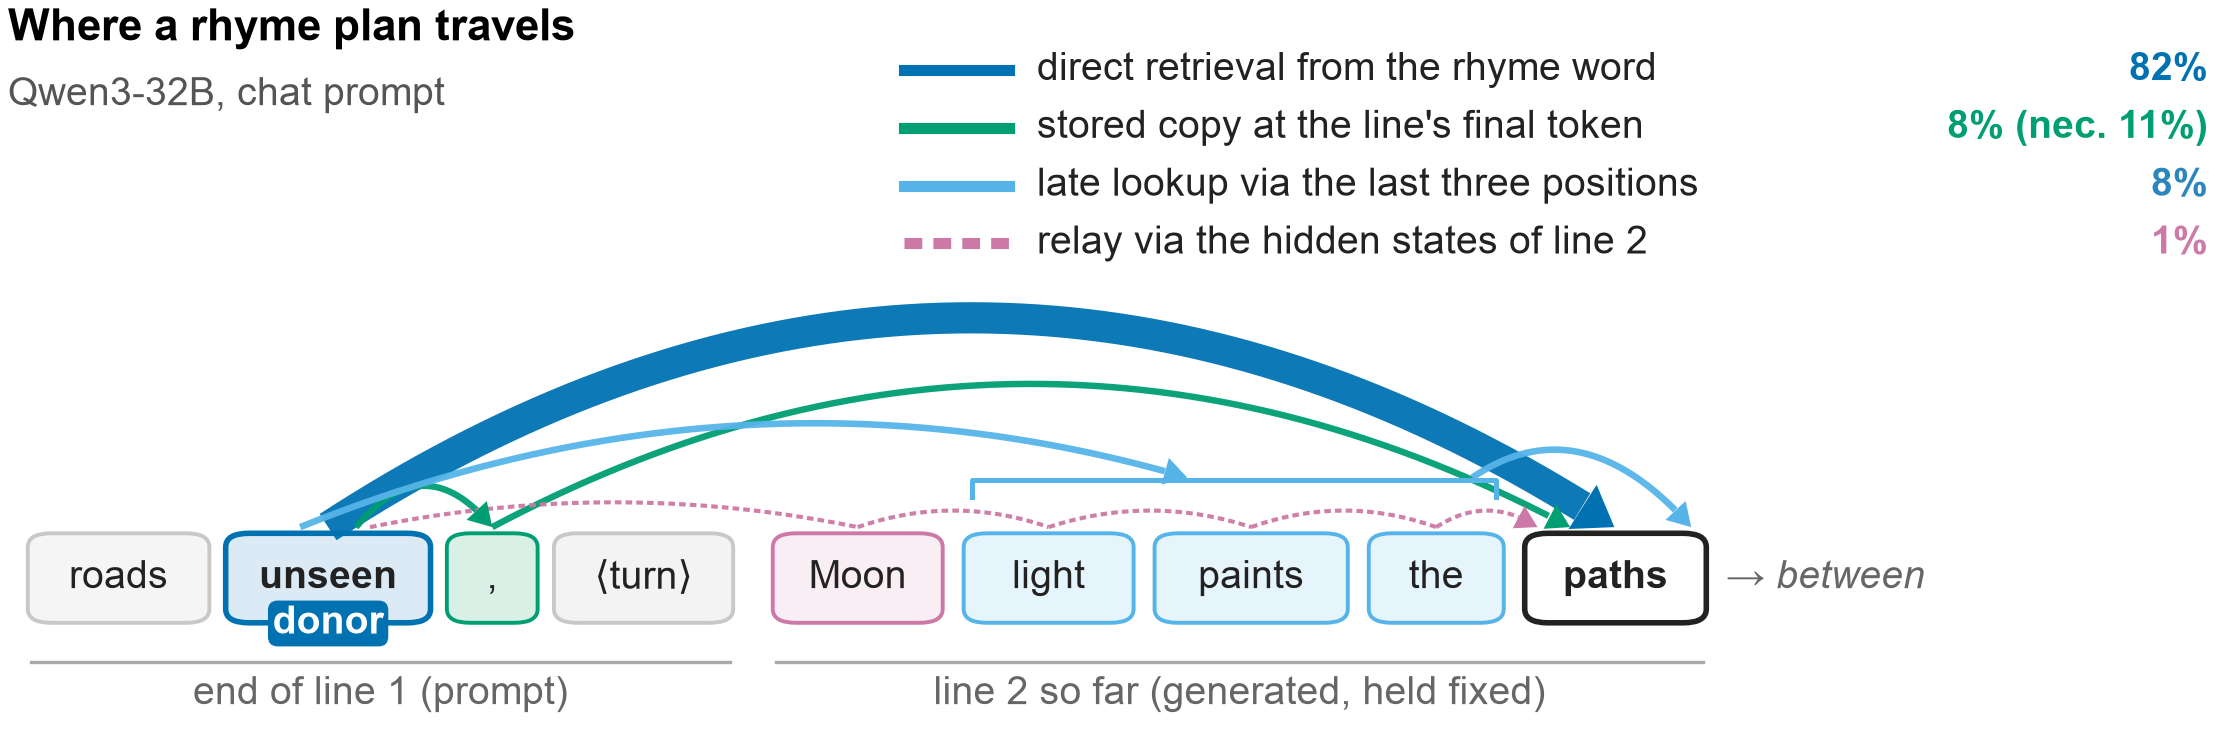
\includegraphics[width=1\linewidth,height=\textheight,keepaspectratio]{manuscript/figures/iclr_fig1_overview.png}

}

\caption{\label{fig-overview}Route accounting on a rhyme plan. The paths
by which a plan formed at the rhyme word of line 1 (where the donor
state is written) reaches the position that predicts the rhyme, with the
line-2 words held fixed. Widths are each path's measured share of
persistence in Qwen3-32B with the chat prompt: most of the plan is read
directly from the rhyme word, and relay through the hidden states of
line 2 accounts for 1\%. Appendix Figure~\ref{fig-overview-points}
gives, for every setting and model, the looked-up share and the share of
relay or of an unsplit indirect path.}

\end{figure}%

We introduce \textbf{route accounting} (Section~\ref{sec-method}). A
donor's hidden states are written at the source positions, and the
effect is measured where the information is used. Fixing the generated
text separates emission from persistence. Clamping the states of chosen
groups of positions, at every layer, separates direct retrieval of the
source from indirect paths through intermediate positions, which we
split by position into the stored copy, the late lookup just before the
target, and relay through the rest of the generated text. Direct
retrieval, the stored copy and the late lookup all read the information
from a fixed prompt position, so they are the three forms of lookup;
relay is the only path that holds it across the generated text. On
induction \citep{olsson2022induction}, where the known mechanism passes
information through the hidden state at the position of a copied token,
route accounting finds that indirect path as the largest path in all
nine models tested (Section~\ref{sec-control}).

Applied to four tasks in 15 checkpoints from three model families, route
accounting finds one principle, within the settings tested (short
generated spans, thinking disabled): \textbf{lookup, not relay}. Models
read unwritten information near the point of use from a fixed position
of the prompt, the source or a copy stored next to it, rather than relay
it through the hidden states of the text they generate
(Table~\ref{tbl-map}; Section~\ref{sec-lookup}). Rhyme plans are read
mainly from the rhyme word (68 to 95\% of persistence in all but one
configuration), and relay accounts for at most 1\% in all 21 runs. Donor
states at every position after a computed value's source move the answer
by at most 4.9\% (variable chains) and 6.4\% (sums) of the source
effect, while written intermediate values are followed: emission
accounts for at least 83\% of the effect.

Three stress tests with committed decision rules make relay useful or
the content invisible (Section~\ref{sec-stress}). Beyond Gemma 3's
attention window, Gemma 3 27B hands the plan from the rhyme word to the
stored copy, and the generated text accounts for 9 to 13\%, not split
into late lookup and relay. In a recurrent hybrid, entry through the
recurrent layers produces 2 to 4\% of persistence. A secret choice is
stored at a few low-content prompt tokens, and at most 2\% of its effect
passes through the hidden states of the intervening sentence. The one
path that grows is the stored copy: it appears at 14B and above in Qwen3
and at 12B to 27B in Gemma 3, is present in base checkpoints, and
reconciles published accounts of where the rhyme plan lives.

\textbf{Contributions.} (1) Route accounting, a position-level
decomposition of intervention effects into emission, lookup and relay,
validated on a positive control. (2) The principle that unwritten
information is looked up, not relayed, across tasks, families, sizes,
prompt formats, checkpoints and intervention types. (3) Three stress
tests with committed decision rules that bound it. (4) A stored copy
that emerges with scale, reconciling published accounts of rhyme
planning.

\begin{table}[t]

\caption{\label{tbl-map}Where unwritten information travels: the share
of the effect by path, as a range over the models tested, of persistence
unless stated. \emph{Looked up}: the target reads the source, a copy
stored at a structural token next to it, or the late lookup.
\emph{Relay, or an unsplit indirect path}: relay where it was separated
(rhyme plans); otherwise the named group of intermediate positions.
\emph{Visible} content can be recovered by a reader of the text;
\emph{hidden} content cannot. Dashes mark cells the design rules out. A
share above 100\% means that the other paths, or their interaction, are
negative. The sections and appendix give the full results with 95\%
intervals.}

\centering{

\footnotesize
\setlength{\tabcolsep}{4pt}
\renewcommand{\arraystretch}{1.15}
\begin{tabular}{@{}>{\raggedright\arraybackslash}p{2.35cm}>{\raggedright\arraybackslash}p{2.1cm}>{\raggedright\arraybackslash}p{4.75cm}>{\raggedright\arraybackslash}p{3.75cm}@{}}
\toprule
Content (observability) & Emission & Looked up: direct retrieval, stored copy or late lookup & Relay, or an unsplit indirect path\\
\midrule
Rhyme plan (visible) & 13--25\% of the total effect & rhyme word 68--95\% of persistence (exception: 19\% in Gemma~3 27B, plain, where the stored copy is 37\% by sufficiency and 74\% by necessity); stored copy otherwise 0--16\% by sufficiency; late lookup 1--13\% & relay $\le$1\%\\
Rhyme plan after 500--2,000 filler tokens (Gemma~3 27B) & -- & rhyme word 40--64\%; stored copy necessary for 25--49\% & through the generated text, late lookup and relay together: 9--13\%\\
Computed value, unwritten (visible) & -- & source edits effective; downstream patch effect near zero & every later position together: $\le$4.9\% of the source effect (chains), $\le$6.4\% (sums)\\
Computed value, written (visible) & 83--101\% & bypass to the source $-1$--17\% & --\\
Secret choice (hidden) & no measurable effect (the sentence never names it) & pick-specific information stored after the list: 0--40\% of the text-swap reference, read directly at the reveal (Gemma~4 31B stores 82--91\%; its path split was not run); the rest not reproduced by the post-list patch & through the sentence: $\le$2\% of the text swap ($\le$16\% of the stored part); sentence positions $\le$8\% (Qwen3.5 hybrids)\\
\midrule
Induction (positive control) & -- & direct retrieval $\le$3\% (10--31\% in Qwen3-32B and the Qwen3.5 hybrids) & through the copied token's position (prompt): 53--137\%\\
\bottomrule
\end{tabular}

}

\end{table}%

\section{Route accounting}\label{sec-method}

\textbf{Setting.} A model processes a prompt and generates text. An
intervention changes the information at a set of \textbf{source}
positions \(S\), and its effect is measured at a later \textbf{target}
position \(t\) where that information is used. The positions strictly
between them, \(M\), include the end of the prompt and the tokens
generated so far. Every intervention is an \textbf{all-layer state
edit}: the residual stream at every layer of each source position is
replaced by the states of a \emph{donor} prompt that differs only in the
content under study (a first line with a different rhyme, a list in a
different order), while the prompt text is unchanged. The outcome is a
log-odds contrast at the target,

\[
R \;=\; \log \sum_{v\in\mathcal V_{\rm donor}} p(v\mid\cdot) \;-\; \log \sum_{v\in\mathcal V_{\rm orig}} p(v\mid\cdot),
\]

where \(\mathcal V_{\rm donor}\) and \(\mathcal V_{\rm orig}\) are the
tokens consistent with the donor's and the original content, for example
the single-token perfect rhymes of each rhyme word. Effects are changes
in \(R\) relative to the unedited run; positive values move the target
toward the donor.

\textbf{Emission and persistence.} The edit can change what the model
writes, and the written tokens are read back. Let \(g_0\) and \(g_1\) be
the texts generated with the edit off and on, and \(R(i,g)\) the outcome
with the edit in state \(i\in\{0,1\}\) and the text fixed to \(g\). Then

\[
\underbrace{R(1,g_1)-R(0,g_0)}_{\text{total}}
\;=\;
\underbrace{R(0,g_1)-R(0,g_0)}_{\text{emission}}
\;+\;
\underbrace{R(1,g_1)-R(0,g_1)}_{\text{persistence}} .
\]

\textbf{Emission} replays the edited words with the edit off.
\textbf{Persistence} is what the edit does with the text held fixed. We
also report persistence with the original text, \(R(1,g_0)-R(0,g_0)\),
the other order of the decomposition, where the two differ (Appendix
Section~\ref{sec-app-sixcell} gives the single-token form).

\textbf{Paths within persistence.} The target can read the edited source
itself (\textbf{direct retrieval}), or the hidden states of intermediate
positions can read it and pass it on (an \textbf{indirect path}). We
separate the two by clamping states. Let \(h^{0}\) and \(h^{1}\) be the
per-layer states of the clean and the edited run, both with the text
fixed, and write \(R[\,S\!\leftarrow\!a,\;G\!\leftarrow\!b\,]\) for the
outcome when the source receives the states of run \(a\) and a group
\(G\subseteq M\) those of run \(b\), at every layer, with all other
positions recomputed. With \(R_0\) the clean outcome,

\[
\begin{aligned}
P &= R[S\!\leftarrow\!1] - R_0 &&\text{persistence,}\\
D &= R[S\!\leftarrow\!1,\;M\!\leftarrow\!0] - R_0 &&\text{direct retrieval (every intermediate position clean),}\\
T &= R[M\!\leftarrow\!1] - R_0 &&\text{indirect paths (source clean, intermediates as in the edited run),}\\
\Delta &= P - D - T &&\text{interaction (additivity gap).}
\end{aligned}
\]

Because the intermediate states are overwritten at every layer, \(D\)
reaches the target only through its own attention to the source, and
\(T\) only through intermediate positions. For a group \(G\) we report
its \textbf{interventional sufficiency},
\(\mathrm{Suf}(G)=R[G\!\leftarrow\!1]-R_0\), the effect of the group
alone, and its \textbf{interventional necessity},
\(\mathrm{Nec}(G)=P-\big(R[S\!\leftarrow\!1,\,G\!\leftarrow\!0]-R_0\big)\),
the loss of persistence when the group alone is reset to its clean
states. When paths combine additively, the two agree and shares
partition the effect. Where the interaction is large (at most 33\% of
persistence, in Gemma 3 27B couplets), shares are not exclusive, and we
report both measures and their average, the two-player Shapley value
\citep{shapley1953}. Shares are divided by the persistence of the same
run unless another denominator is named, and intervals are
item-bootstrap 95\% intervals \citep{efron1994bootstrap}.

\textbf{Path names.} We split \(M\) into three groups by position, not
by any hypothesis about their content, and name the indirect path
through each. The \textbf{stored copy} passes through the prompt
positions right after the source line (in couplets, the token that ends
line 1 and the chat template). The \textbf{late lookup} passes through
the three positions just before the target; it is the late retrieval of
\citet{hanna2026latent} read in two steps. \textbf{Relay} passes through
the remaining positions of the generated text; it is the path monitoring
is concerned with. Because the text is held fixed, every indirect path,
relay included, passes information only in hidden states; information in
the written words themselves is emission. Information is \textbf{looked
up} when it arrives by direct retrieval, the stored copy or the late
lookup. Where a group was not split further, we name it and call its
effect the indirect path through it.

\subsection{Positive control: induction}\label{sec-control}

A decomposition that never reports an indirect path could be blind to
one. In a repeated sequence \(\ldots A\,B\ldots A\), a previous-token
head writes ``preceded by \(A\)'' into the position of \(B\), and an
induction head at the second \(A\) finds that position and copies \(B\)
\citep{olsson2022induction}. Information about the first \(A\) therefore
reaches the prediction through the hidden state of an intermediate
position, while the token \(B\) itself is unchanged. We edit the first
\(A\) in 100 random sequences and measure \(\log p(B)\) at the second
\(A\). The committed criterion (an indirect path above 80\% of
persistence, direct retrieval near zero) holds cleanly in Qwen3 1.7B to
14B (indirect path 108 to 137\%, the excess an interaction; direct
retrieval 1 to 3\%). It holds partly in Gemma 3 12B and 27B, where
conflicting edited positions lower the all-position cell to 53 to 55\%,
and in Qwen3-32B and the Qwen3.5 hybrids, which also read the source
directly (10 to 31\%). In every model the indirect path is the largest
path (Appendix Section~\ref{sec-app-control}). The key position lies
right after the source, so this path resembles a stored copy more than
relay; but with the generated text fixed, generated tokens are ordinary
context positions, and the clamp is the same operation at any position.
The lookup-dominated results that follow are therefore informative
negatives, not a blind spot of the method.

\textbf{Models and protocol.} We study Qwen3 1.7B to 32B
\citep{yang2025qwen3}, Gemma 3 1B to 27B \citep{gemma3}, the recurrent
hybrids Qwen3.5 4B, 9B and 27B \citep{qwen2026qwen35}, and Gemma 4 31B
\citep{gemma4} for the hidden choice, as instruction-tuned checkpoints
with base checkpoints as checks and thinking disabled. After the initial
couplet split, the design and decision rule of every experiment were
committed to the repository before its first result, and later additions
are labelled post hoc (Appendix Section~\ref{sec-app-prereg}; materials
in Appendix Section~\ref{sec-app-materials}).

\section{Unwritten information is looked up}\label{sec-lookup}

\subsection{Rhyme plans}\label{sec-couplets}

Rhyming couplets are the flagship case of latent planning
\citep{lindsey2025biology, hanna2026latent}. We use the couplet prompts
of \citet{hanna2026latent} in their chat format and repeat every run
with the plain prompt of \citet{ma2026plan}, which has no chat template.
\emph{Chat} and \emph{plain} name prompt formats, not checkpoints:
instruction-tuned models are run with both, and base checkpoints, which
have no chat template, with the plain prompt only (100 couplets per run;
Appendix Section~\ref{sec-app-couplets}). The source is the last word of
line 1, the donor a couplet from a different rhyme group, and the target
the position that predicts the first token of line 2's last word, with
the line-2 prefix fixed. The edit moves line 2 off its rhyme (at most
2\% of second lines still rhyme with the original, against 83 to 100\%
before the edit) and onto the donor's rhyme in 27 to 95\% of couplets.
The emitted line-2 words account for 13 to 25\% of the total effect; the
rest is persistence.

\textbf{Direct retrieval dominates, and relay is at most 1\%.}
Figure~\ref{fig-couplets} decomposes persistence in all 21 runs. Direct
retrieval of the rhyme word accounts for 76 to 95\% of persistence in
every Qwen3 configuration (1.7B to 32B, chat and plain, instruct and
base) and 80 to 95\% in Gemma 3 1B to 12B. The late lookup accounts for
1 to 13\%. Relay through the rest of the generated line is at most 1\%
of persistence in every run, by sufficiency in all 21 and by necessity
in the 17 where it was measured. Before running the larger models we
committed two criteria for the claim that relay grows with scale: the
indirect share must rise with log parameter count across Qwen3 1.7B to
32B, and the rise must come from relay. The first holds (6.2 percentage
points per decade, 95\% interval {[}2.8, 9.6{]}); the second fails
(relay is \(-0.06\) to \(+0.16\), against persistence of 12 to 26). The
indirect share grows as the late lookup up to 8B and as the stored copy
from 14B. Controls support the split (Appendix
Section~\ref{sec-app-couplets}): same-rhyme donors leave the rhyme
almost unchanged, the rhyme word matters two to three times more than
any other position of line 1, and the published feature steering of
\citet{hanna2026latent} gives the same split as the state edit (direct
retrieval 90, 88 and 84\% at 4B, 8B and 14B, against 91, 90 and 82\%).

\begin{figure}[t]

\centering{

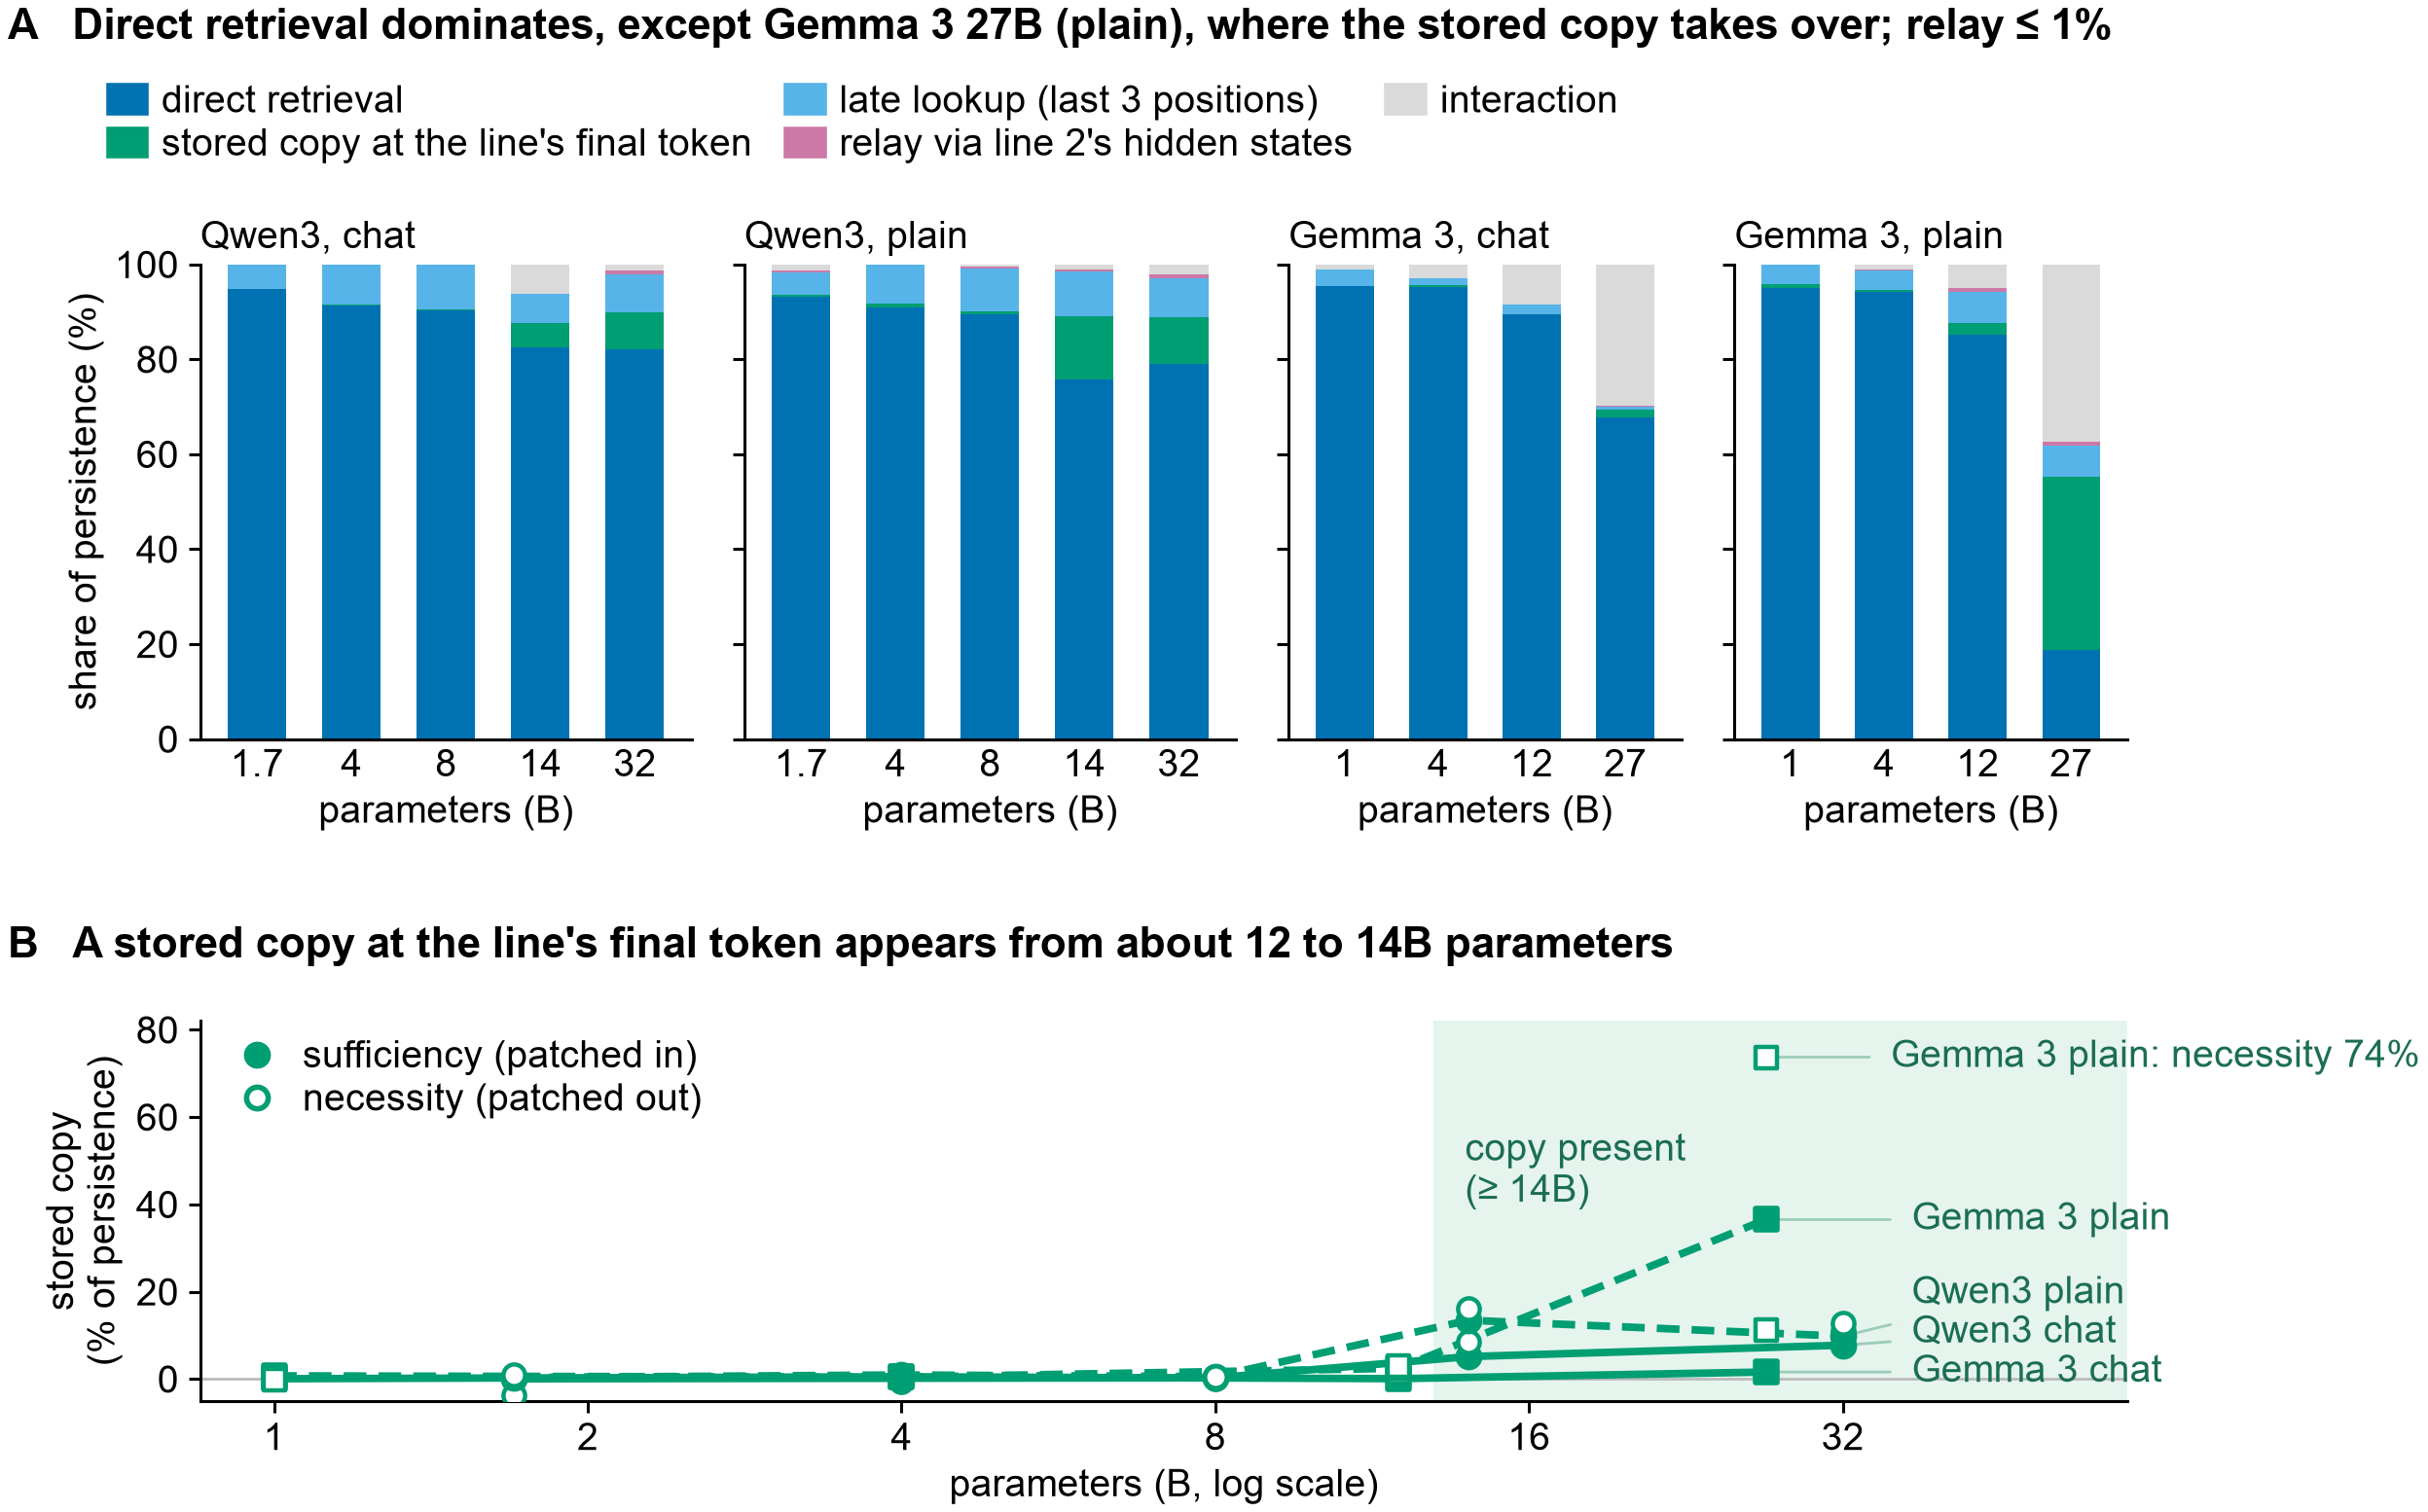
\includegraphics[width=1\linewidth,height=\textheight,keepaspectratio]{manuscript/figures/iclr_fig2_couplet_routes.png}

}

\caption{\label{fig-couplets}Couplet paths across scale, family and
prompt format (100 couplets per run; instruction-tuned checkpoints;
Appendix Table~\ref{tbl-storage} adds the base checkpoints).
\textbf{Top:} composition of persistence from the sufficiency cells:
direct retrieval of the rhyme word (blue), the stored copy at the line's
final token (green), the late lookup (light blue), relay through the
rest of line 2 (purple; at most 1\%, so barely visible) and interaction
(grey), one bar per model. \textbf{Bottom:} the stored copy's share of
persistence against model size (log scale), by sufficiency (filled) and
necessity (hollow). It is absent up to 8B and present from 14B in Qwen3
and at 12B to 27B in Gemma 3.}

\end{figure}%

\subsection{The stored copy}\label{sec-storage}

Gemma 3 27B is the exception to the dominance of direct retrieval.
Direct retrieval falls to 68\% of persistence with the chat prompt and
19\% with the plain prompt, and two components appear: a large
interaction and a copy stored at the line's final token.

\textbf{It sits on the line's final token.} Resetting the tokens between
the rhyme word and line 2 one at a time locates the copy. In all five
runs analysed, the line's final token accounts for 90 to 100\% of these
tokens' summed necessity, and the chat-template tokens hold almost
nothing (Appendix Figure~\ref{fig-sites}). With the chat prompt this
token is the comma that ends line 1; with the plain prompt, the newline.
The site is the last token of the line, whatever that token is; in the
prompt of \citet{lindsey2025biology} it is the newline, where they
observed Claude's rhyme plan being formed.

\textbf{It emerges with scale, before instruction tuning.} In Qwen3 the
copy is absent up to 8B (necessity at most 0.9\% of persistence) and
appears at 14B (8\% with the chat prompt and 16\% with the plain prompt,
by necessity), remaining at 32B (11\% and 13\%). In Gemma 3 it is small
at 12B (1 to 3\%) and present at 27B: 11\% by necessity with the chat
prompt and, with the plain prompt, 37\% by sufficiency and 74\% by
necessity, more than is read from the rhyme word (19\%), while relay
stays at 1\%. The base checkpoints we tested have the copy wherever the
matching instruct model does (Qwen3-14B-Base 16\% against 13\%; Gemma 3
12B PT 5\% against 2\%), so it most likely arises in pretraining.
Same-rhyme donors remove it, so it encodes the rhyme.

\textbf{Where paths interact, sufficiency understates it.} In Gemma 3
27B with the chat prompt, the copy alone moves the rhyme by only
\(+0.68\), yet resetting it removes \(+4.87\) {[}3.18, 6.73{]} of a
persistence of \(+43.1\); the interaction is 29\% of persistence (Qwen3
at most 5\%). The target combines the rhyme word and the copy, and reads
conflicting evidence when only one of them is edited: the copy is a
redundant second lookup site.

\textbf{Reconciling published accounts.} The heads near the end of line
2 that read the rhyme word \citep{hanna2026latent} are direct retrieval
with the late lookup; the plan found and steered at the end of line 1
\citep{lindsey2025biology, maar2026plan} is the stored copy of larger
models; the hand-off to the newline in Gemma 3 27B only
\citep{ma2026plan} matches our plain-format result; and no copy appears
below 8B, consistent with the inert newline that
\citet{jacopin2026improvisation} finds at 0.6B to 2.6B. Each account is
correct for the configuration it studies (Appendix
Section~\ref{sec-app-couplets}).

\textbf{Why the stored copy is a lookup, not relay.} It passes through
an intermediate position, but it is a fixed structural token next to the
source. The copy is written there once, read directly however much text
intervenes, and does not move with generation. It never travels through
the hidden states of the generated text, so a monitor probing hidden
states can find it at a known prompt position.

\subsection{Computed values}\label{sec-computed}

Computed information is not present at any single token, which is where
an indirect path would seem most useful (Appendix
Section~\ref{sec-app-computed}). In two-digit sums (Qwen3 1.7B to 32B,
104 items, a filler of 0 to 32 tokens before the answer), donor states
at every position from the question mark to the answer move the answer
by at most 6.4\% of the effect of donor operand digits. Variable chains
(\texttt{a\ =\ 23}, \texttt{b\ =\ a\ +\ 4}, \ldots,
\texttt{What\ is\ e?}) make recomputation at the answer costly and an
indirect path, passing the running value from statement to statement,
the natural one, so we designed them as a second positive-control
candidate for an indirect path. They are not one. Donor states at every
position after the starting value together, a test that would detect a
running value stored redundantly, move the answer by at most 4.9\% of
the effect of editing the starting value (32B, one update), and their
interval includes zero at every size with five updates, where a running
value would help most. This is consistent with the answer re-reading its
visible sources; recomputation itself is not measured.

\subsection{Written values}\label{sec-emission}

When asked to compute each variable in order, the model writes the
donor's values in 86 to 100\% of items, and the answer follows the text.
With the chain cut before its last value, emission accounts for 83 to
101\% of the effect at 1.7B to 32B, and the bypass that re-reads the
source stays below 17\% (the 101\%, at 32B with five updates, reflects a
slightly negative bypass). For a binary mediator such as the article
\emph{a} or \emph{an} before a planned noun, emission factorizes exactly
into the change in what is written times the written token's
\textbf{leverage}, how much it matters to what follows (Appendix
Section~\ref{sec-app-computed}). For the a/an planning features of
\citet{hanna2026latent} in Qwen3-4B, 92 to 94\% of their
feature-specific effect on the planned noun travels through the
generated article, the bypass is at the level of random features, and
the effect through the article scales with leverage.

\section{Settings built to favour relay}\label{sec-stress}

Relay is not required when every layer can read every earlier position
and the content is visible. We therefore run three stress tests that
remove one of these conditions, each with a decision rule committed
before its first result (Figure~\ref{fig-stress}; Appendix
Section~\ref{sec-app-prereg}, Section~\ref{sec-app-stress} and
Section~\ref{sec-app-hidden}).

\begin{figure}[t]

\centering{

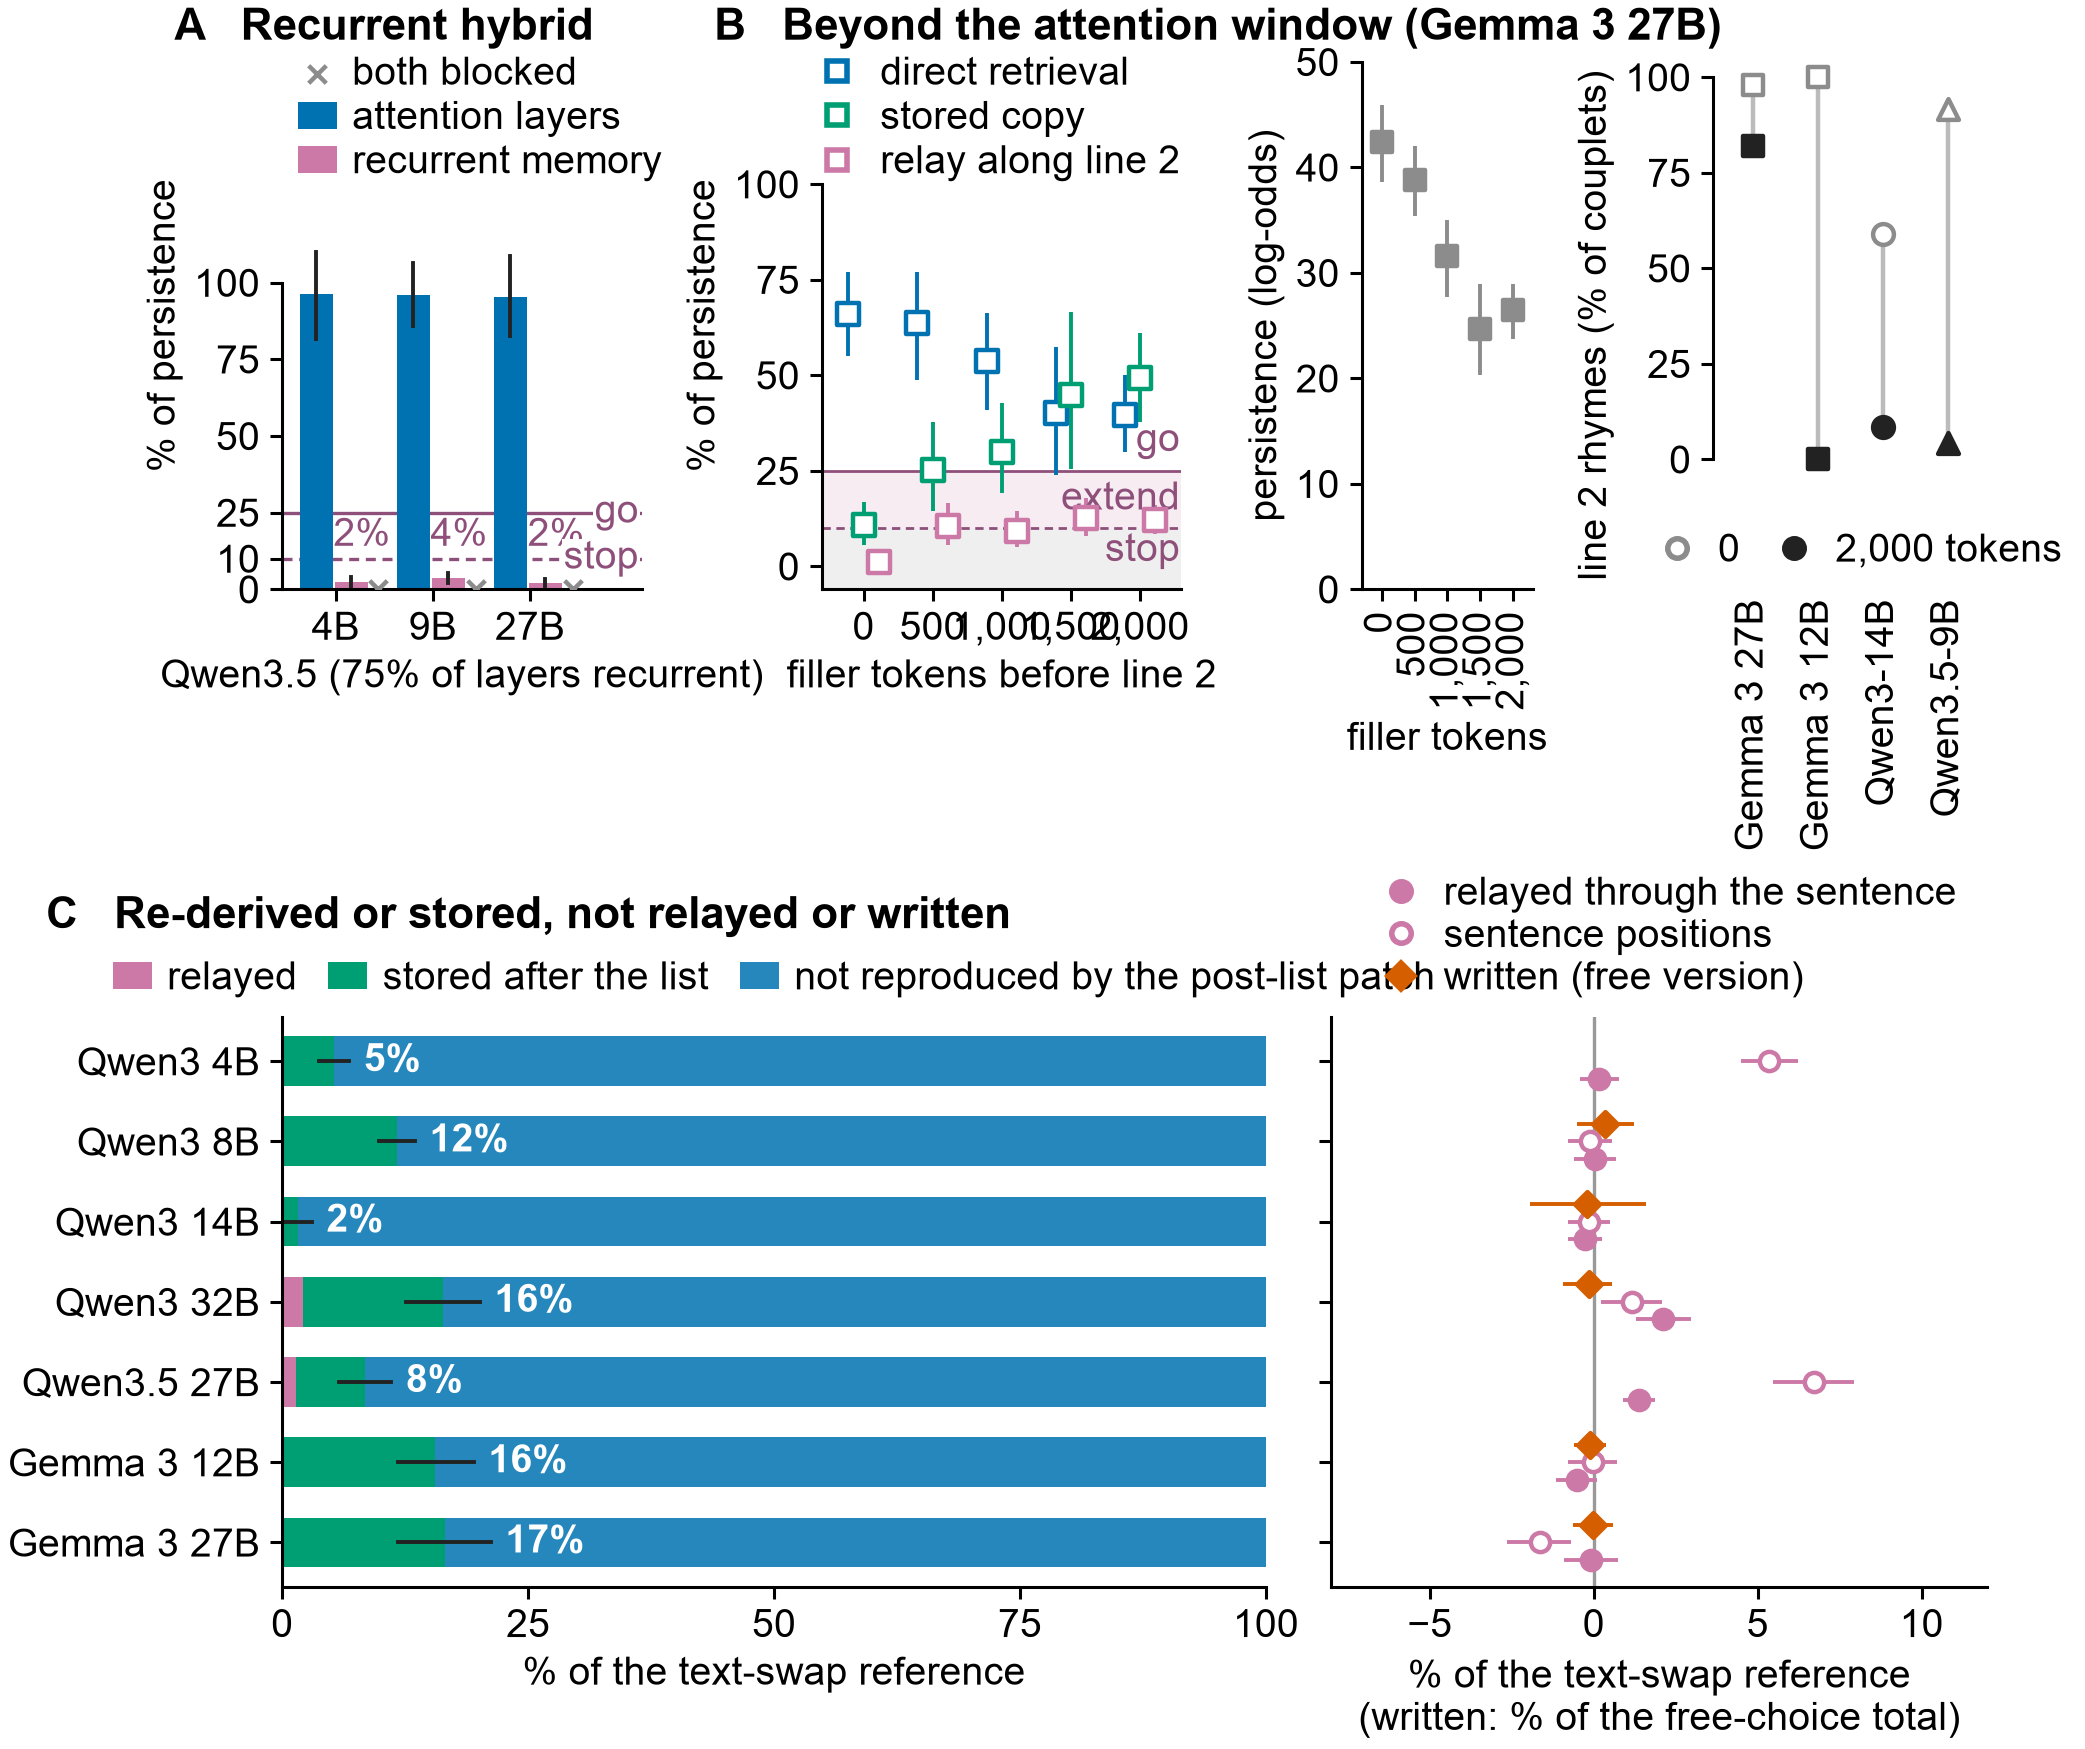
\includegraphics[width=1\linewidth,height=\textheight,keepaspectratio]{manuscript/figures/iclr_fig4_stress_tests.png}

}

\caption{\label{fig-stress}In settings built to favour relay, models
still look up information. \textbf{A:} Gemma 3 27B with filler between
line 1 and line 2 (couplets per distance in brackets; the dotted line
marks where line 1 leaves the 1,024-token window). Direct retrieval
falls while the stored copy becomes necessary for about half of
persistence; the generated text (the cue and line 2, not split into late
lookup and relay) is 9 to 13\%, between the committed stop and go lines.
Side panels: absolute persistence, and for four unedited models the
share of couplets whose line 2 still rhymes, with no filler (open) and
after 2,000 filler tokens (filled). \textbf{B:} Qwen3.5 hybrids (three
of every four layers recurrent), with the donor state allowed to enter
only one layer type at the source. Entry through the attention layers
accounts for nearly all of persistence; entry through the recurrent
layers produces 2 to 4\%, below the committed stop line (10\%).
\textbf{C:} hidden choice, as shares of the text-swap reference: not
reproduced by the post-list patch, stored after the list, and passed
through the sentence. The right subpanel shares the bars' rows and
magnifies, with 95\% intervals, the indirect path through the sentence,
the pick held at the sentence positions, and emission through a sentence
the model writes (share of that run's total).}

\end{figure}%

\subsection{Beyond the attention window}\label{sec-distance}

Gemma 3 alternates five local sliding-window layers
\citep{beltagy2020longformer} with a 1,024-token window with one global
layer \citep{gemma3}, so once line 1 lies more than 1,024 tokens before
the target, five of six layers cannot read it. We insert up to 2,000
tokens of neutral filler before line 2 and split the indirect path into
the stored copy, the filler and the generated text (the cue and line 2).
The committed decision number was the share of persistence through the
generated text: ``go'' at 25\%, ``stop'' below 10\%, and an extension to
50 couplets in between; a rise counts only if the absolute indirect
effect also grows. At 2,000 tokens Gemma 3 27B still rhymes in 82\% of
couplets, and it hands the plan from the rhyme word to the stored copy
at the line's final token. Direct retrieval falls from 66\% to 40\% of
persistence (\(+28.0\) to \(+10.5\)), while the copy's necessity rises
from 11\% to 49\% (\(+4.6\) to \(+13.0\) {[}10.0, 16.1{]}) although
persistence falls from \(+42.4\) to \(+26.4\); the copy alone moves the
rhyme by \(+0.1\) without filler and by \(+9.7\) with it. The rise is
absolute, so it passes the committed rule; the filler passes on nothing.
The generated text rises from 1\% to about 11\% by sufficiency as soon
as filler is present (12\% at 2,000 tokens, \(+3.2\) {[}2.2, 4.3{]}) and
does not grow further. It includes the last three positions, so it mixes
relay with the late lookup, and it falls between ``stop'' and ``go'':
how much of it is relay remains unresolved. The committed window
prediction is only partly supported: the largest step is where line 1
leaves the window, but the shift begins at 500 tokens. Models without a
strong stored copy (Gemma 3 12B, and Qwen3.5-9B and Qwen3-14B, whose
attention has no window) lose the plan instead, and no indirect path
takes over.

\subsection{Recurrent memory}\label{sec-recurrent}

Qwen3.5 \citep{qwen2026qwen35} interleaves three Gated DeltaNet layers
\citep{yang2025gateddeltanet} with each attention layer. In a recurrent
layer, information from the source can reach a later position only
through a fixed-size state updated position by position, invisible in
the text; the attention layers can still look it up. The test asks which
path the model uses when both are available. In the
\emph{attention-only} cell, the donor state enters at the source but the
input of every recurrent layer there is restored to its clean value; the
\emph{recurrent-only} cell is the converse. The committed rule, decided
on the largest model, was ``go'' if recurrent-only is at least 25\% of
persistence and ``stop'' below 10\%. Recurrent-only is 3\% and 4\% of
persistence at 4B and 9B, and 2\% at 27B (\(+0.41\) {[}0.18, 0.64{]} of
\(+18.8\)); attention-only is 95 to 97\%, and blocking both cancels the
donor on every couplet. Decision: stop. The design controls which layer
type receives the donor at the source, not every later path through each
type, so it bounds donor entry through recurrent memory at 2 to 4\% of
persistence.

\subsection{Hidden content}\label{sec-hidden}

A choice that no reader can infer from the text is the case monitoring
cares about most. The prompt reads: ``Secretly choose one fruit from
this list: \{4 fruits\}. Do not write your choice yet. First write one
sentence about the weather. Then write the fruit you chose.'' The greedy
pick depends on the model's preferences and the list order, so no reader
can compute it. The donor is the list in another order with a different
pick; the reference is a \emph{text swap} that writes that order into
the prompt. In Qwen3-8B and Gemma 3 12B and 27B, donor states at the
positions after the list move the reveal by 12 to 16\% of the text swap,
all of it read directly; the part that passes through the sentence is
zero within its interval, and the rest of the pick is presumably
re-derived at the reveal from the visible list. In Qwen3-32B and the
Qwen3.5 hybrids the indirect path through the sentence is small but
nonzero: at most 2\% of the text swap, but one eighth to one fifth of
the stored part. A sentence the model writes itself never names an item
and has no measurable effect on the reveal (emission \(-0.01\) to
\(+0.02\)).

\textbf{The stored signal is pick-specific and sits at predictable
tokens.} In an out-of-list control, the donor's pick does not occur in
the prompt, yet post-list donor states raise it more than the donor's
other items. This \emph{pick specificity}, added post hoc for fruits,
was then committed as the primary measure of a replication with animals,
which confirms it in both families; a donor with the same pick leaves
the preference unchanged. The stored share is larger in Gemma and grows
with generation (Gemma 3 15 to 40\%, Gemma 4 31B 82 to 91\% of the text
swap's pick specificity), and it shrinks with scale in Qwen3 (0 to 7\%
at 14B and 32B). Per-token necessity places it on two or three
low-content tokens: the periods that close the list or the instruction,
and one function word or possessive token of the instruction (in Gemma 3
27B, 77\% on \emph{the} in ``about the weather''). When the instruction
is reworded, the site moves with the wording at 4B, 12B and 27B
(Appendix Figure~\ref{fig-sites}). These controls do not distinguish a
stored pick from a stored copy of the list, so we claim only that
pick-specific information absent from the text is stored after the list
and read at the reveal. As for rhymes, the copy is stored once, at a
segment-closing or predictable token, and read at the point of use.

\section{Related work}\label{sec-related}

\textbf{Planning.} Hidden states carry information about tokens several
positions ahead \citep{pal2023futurelens, men2024lookahead}, much of it
a by-product of current-token computation \citep{wu2024plan}, and
attribution graphs \citep{ameisen2025attribution} expose planning in
rhyming \citep{lindsey2025biology} and article choice
\citep{hanna2026latent}. \citet{hanna2026latent} show that such planning
emerges with scale in Qwen3 and identify the circuit that retrieves the
rhyme plan near the end of line 2; other studies locate or steer the
plan at the line boundary \citep{maar2026plan, ma2026plan}, which
\citet{jacopin2026improvisation} finds inert at 0.6B to 2.6B. These
works ask whether and where a plan exists. We ask which path it takes,
and show that the published accounts measure different lookup sites.

\textbf{Causal mediation and patching.} Route accounting builds on
activation patching and causal mediation
\citep{vig2020mediation, meng2022rome, geiger2025abstraction, chan2022scrubbing, zhang2024patching, heimersheim2024patching}
and is closest to path patching
\citep{wang2023ioi, goldowskydill2023path} and attention knockout
\citep{geva2023recall}. It defines paths over positions rather than
components, separates emission through generated text from persistence,
and reports sufficiency, necessity and interaction side by side, in the
spirit of evaluating mechanisms against explicit mediators
\citep{mueller2026mediator}.

\textbf{Structural tokens.} Label words \citep{wang2023labelwords},
separators \citep{chen2024sepllm} and registers
\citep{darcet2024registers} aggregate information, while attention sinks
absorb surplus attention \citep{xiao2024sinks}; the stored copies we
find are causal instances that grow with scale and distance.

\textbf{Chain-of-thought faithfulness and monitoring.} Written reasoning
can be unfaithful to the computation behind an answer
\citep{turpin2023unfaithful, lanham2023faithfulness, chen2025reasoning};
models can learn to compute with filler tokens \citep{pfau2024dots} and
could in principle encode reasoning steganographically
\citep{roger2023steganography}. Monitoring is valuable but fragile
\citep{korbak2025monitorability, baker2025monitoring}, and more robust
when reasoning is necessary for the task \citep{emmons2025cot}. These
studies measure behaviour; route accounting measures internal paths, and
our hidden choice, unlike secrets installed by training
\citep{cywinski2025taboo}, arises without it.

\section{Discussion}\label{sec-discussion}

\textbf{Implications for monitoring.} In the settings tested, what a
model writes, it uses, in proportion to the leverage of the written
token, and what it does not write, it looks up from a few prompt
positions: the sources and copies stored at structural tokens next to
them. If this extends to other tasks, a monitor of internal state could
focus on those positions and track whether stored copies keep growing
with scale. The advice is weakest where the indirect path through
generated text is largest: 9 to 13\% of persistence after filler, not
yet split into late lookup and relay, and one eighth to one fifth of the
small stored hidden part in Qwen3-32B and the Qwen3.5 hybrids.

\textbf{Why look up rather than relay?} Attention makes any earlier
position readable at every layer, so a later position can compute what
it needs when it needs it. But at a distance the model relies on a
stored copy or loses the plan, and even where three quarters of the
layers can pass a plan forward only through a recurrent state, entry
through the attention layers accounts for nearly all of the effect.
Relay appears disfavoured when lookup is available, not merely unneeded.

\textbf{What would overturn the principle.} Much longer generated text,
thinking enabled, tasks that cannot be recomputed from the prompt, or
training that rewards concealment \citep{baker2025monitoring} could
break it, and pause tokens \citep{goyal2024pause} or continuous latent
reasoning \citep{hao2024coconut} are designed to do what we rarely see.
Route accounting applies to each case.

\subsection{Limitations}\label{sec-limitations}

The generated spans are short, thinking is disabled, and the tasks are
constructed; the principle is established only for them. All-layer state
edits are strong and can take a model off its natural distribution,
which the feature-steering replication and the same-rhyme nulls address
only in part. The hidden-choice controls do not distinguish a stored
pick from a stored copy of the list. The models span 1B to 32B
parameters in three families, with Gemma 4 31B for the hidden choice
only. Recomputation at the answer is inferred, not measured. Five
committed checks were not run, and post hoc elements are labelled
(Appendix Section~\ref{sec-app-prereg}).

\section*{AI use statement}\label{ai-use-statement}
\addcontentsline{toc}{section}{AI use statement}

We used AI coding agents and assistants (Claude, Codex and Cursor)
extensively in this work. They wrote and ran experiment code, managed
jobs on a remote workstation, aggregated results, generated the figures
from the committed result files, and drafted and edited manuscript text.
Research questions, experimental designs and decision rules were
discussed with the agents. After the initial couplet split, every design
and decision rule was committed to version control before the
corresponding result was computed. The authors reviewed the code, the
committed results and every claim in the manuscript. Numbers in the text
were checked against the machine-readable result files, and citations
were checked against their sources. We take responsibility for the final
content of this work, including text, claims and artifacts produced with
the aid of generative AI.

\section*{Ethics statement}\label{ethics-statement}
\addcontentsline{toc}{section}{Ethics statement}

This work studies how openly released language models use information
they have not written. Its aim is to support the monitoring of such
models. It involves no human subjects, personal data or harmful content.
The hidden-choice task elicits harmless secret choices (fruits,
animals). The results locate where content that the text does not reveal
is stored, which is information useful to monitors. We do not see a
plausible route by which it helps a model conceal content. The
limitations section states where the findings may not transfer, notably
to long reasoning with thinking enabled. The discussion notes that
training which rewards concealment is untested.

\section*{Reproducibility statement}\label{reproducibility-statement}
\addcontentsline{toc}{section}{Reproducibility statement}

All experiments use publicly released checkpoints (Appendix
Section~\ref{sec-app-materials}) and public prompts released by
\citeauthor{hanna2026latent}
\citetext{\citeyear{hanna2026latent}; \citealp{hanna2026planningdata}}
(used in their chat format and in the plain template of
\citet{ma2026plan}) or generated with fixed seeds. Upon acceptance we
will release the code and result files on GitHub. That release will
contain, for every experiment, the code, the per-item result rows and
summaries with bootstrap intervals, and the scripts that generate every
figure and table from those files. After the initial couplet split, it
will also contain each design and decision rule as committed before the
corresponding result. The log of committed decision rules (Appendix
Section~\ref{sec-app-prereg}) lists each frozen design, its decision
rule and the outcome. Dated deviations are recorded with each
experiment, and the main ones are listed there. Batched edits and
generation were checked against unbatched reference implementations
(Appendix Section~\ref{sec-app-materials}). Compute is described in
Appendix Section~\ref{sec-app-compute}.

\section*{References}\label{references}
\addcontentsline{toc}{section}{References}

\renewcommand{\bibsection}{}
\bibliography{manuscript/references.bib}

\appendix

\setcounter{figure}{0}
\renewcommand{\thefigure}{A\arabic{figure}}
\setcounter{table}{0}
\renewcommand{\thetable}{A\arabic{table}}

\section{All settings at a glance}\label{sec-app-overview}

\begin{figure}

\centering{

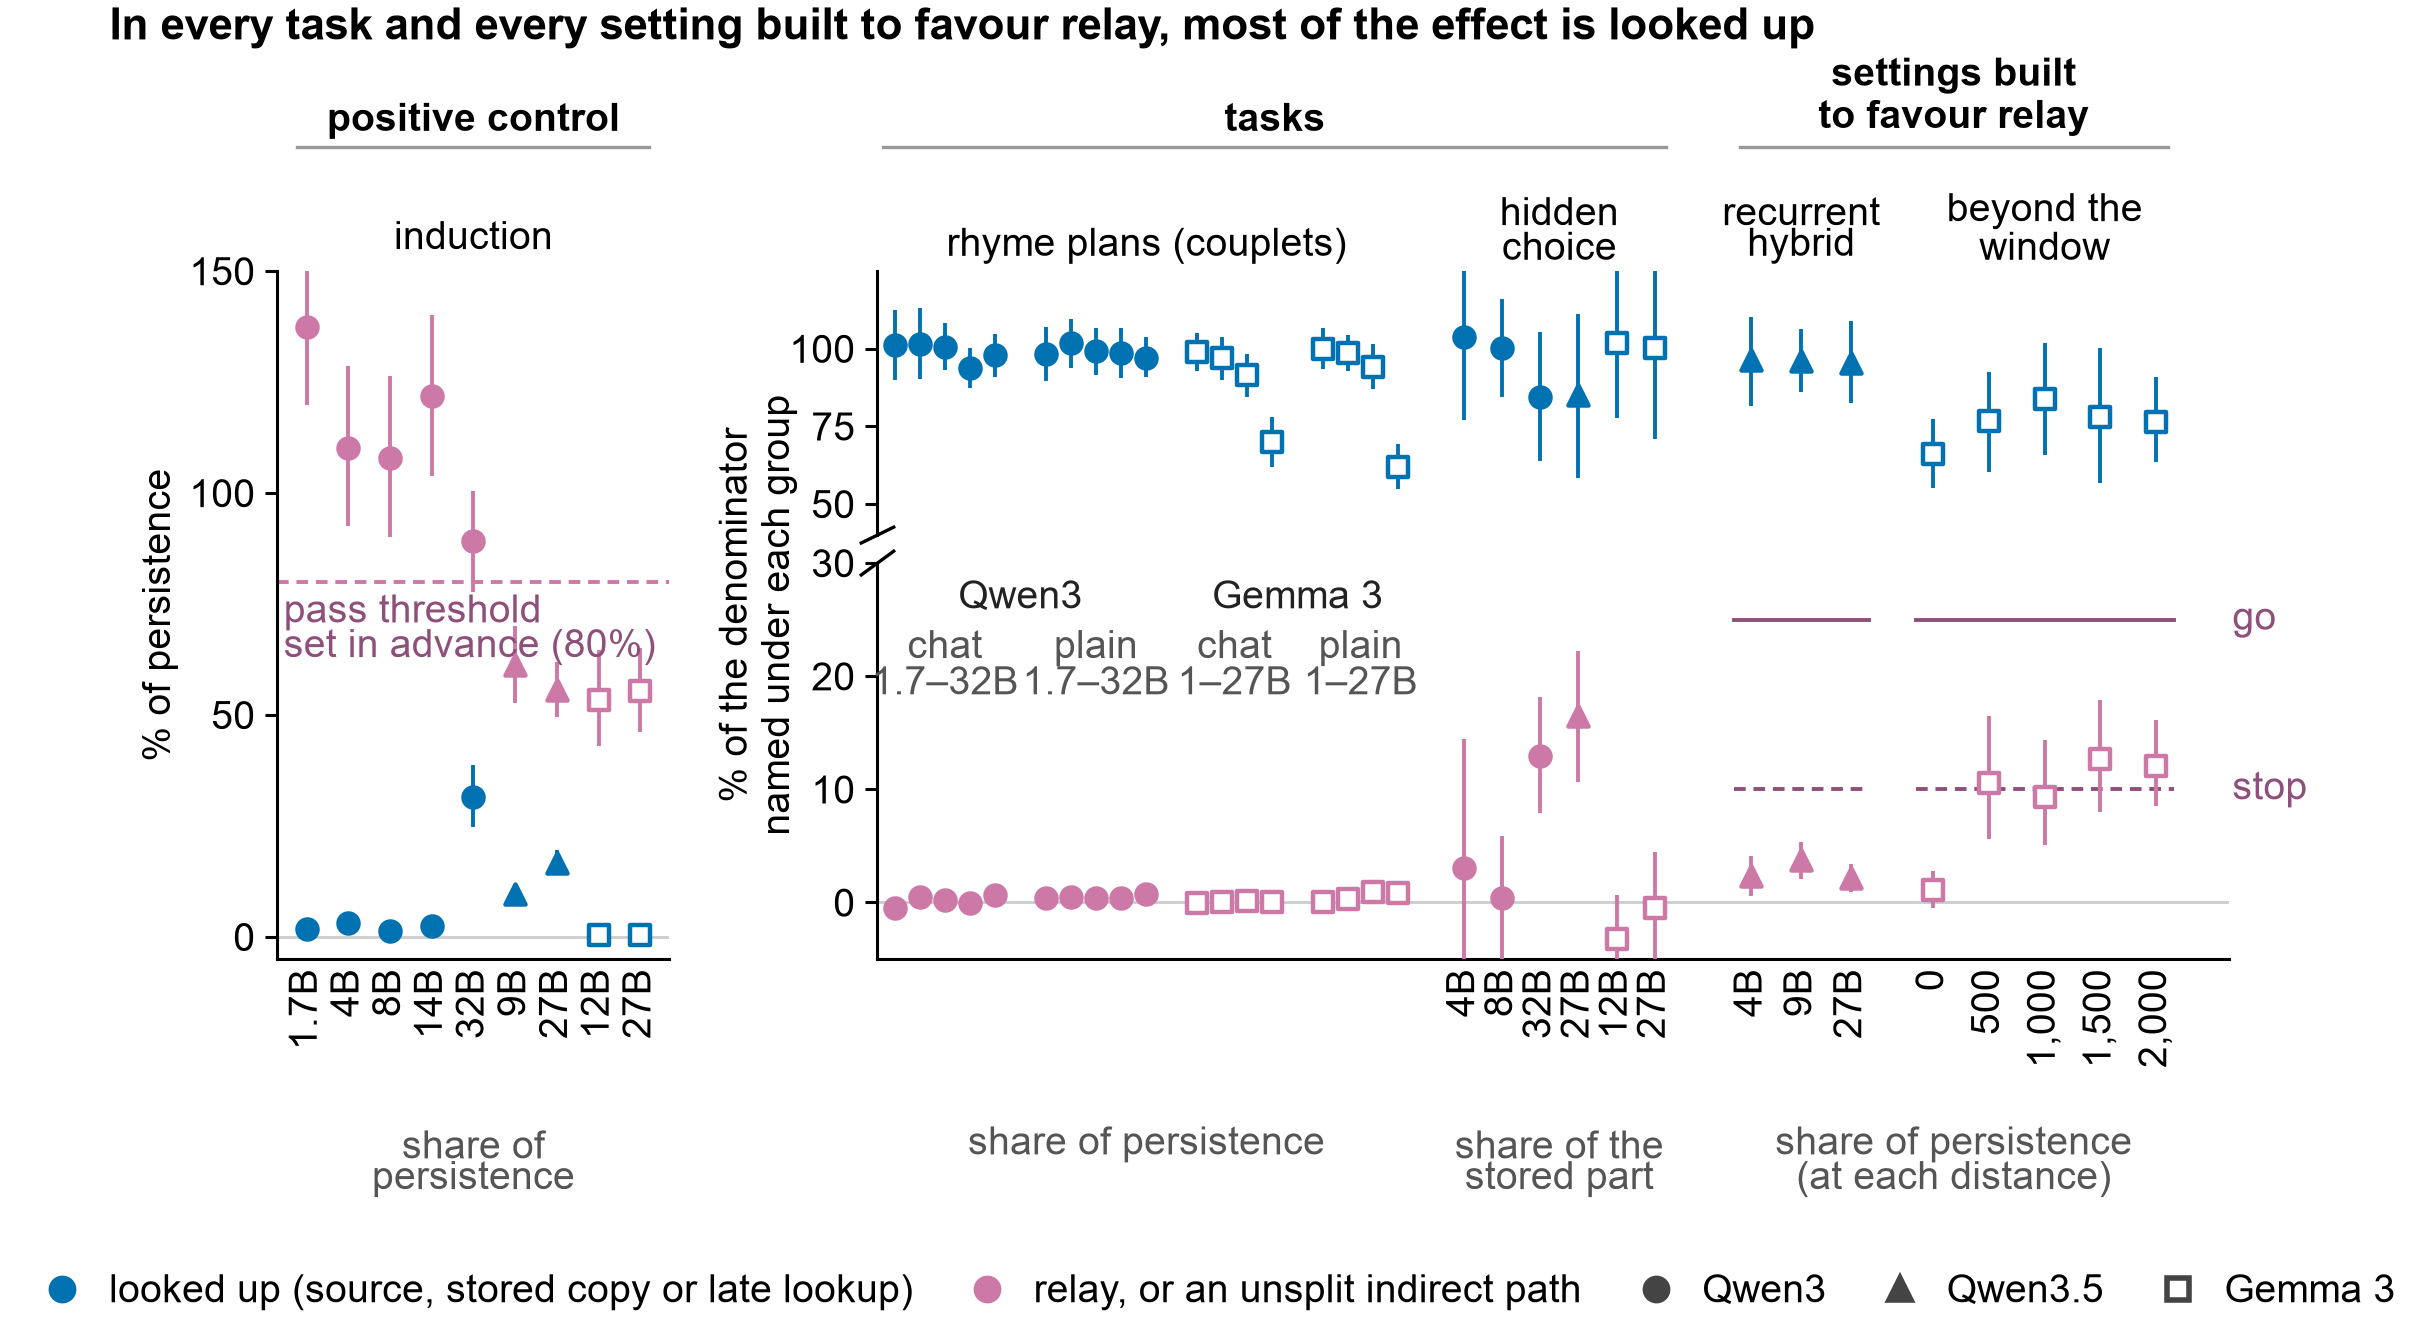
\includegraphics[width=1\linewidth,height=\textheight,keepaspectratio]{manuscript/figures/iclr_figA_overview_points.png}

}

\caption{\label{fig-overview-points}In every task and stress test, most
of the effect is looked up. For every setting and model: the share of
the effect that is looked up (blue) and the share that is relayed, or
takes an indirect path not split further (purple), with 95\% intervals.
The positive control has its own axis (0 to 150\%), with the pass
threshold set before the experiment (an indirect path above 80\% of
persistence). The other settings share a broken axis: looked-up shares
on the upper segment, purple shares on the lower segment (to 30\%), with
the committed stop (10\%) and go (25\%) lines of the stress tests. The
group of intermediate positions and the denominator are given under each
group; for the recurrent hybrid, blue and purple are the shares entering
through the attention and the recurrent layers; Qwen3 is shown filled,
Qwen3.5 as triangles, Gemma 3 open. In the positive control, where an
indirect path is the known mechanism, route accounting finds it as the
largest path, so the small purple shares elsewhere are not a blind spot
of the method. Interactions are reported in the sections.}

\end{figure}%

\section{Models and materials}\label{sec-app-materials}

\textbf{Models.} Qwen3 1.7B, 4B, 8B, 14B and 32B
(\texttt{Qwen/Qwen3-*}), and Qwen3 8B and 14B base
(\texttt{Qwen/Qwen3-*-Base}). Gemma 3 1B, 4B, 12B and 27B
instruction-tuned (\texttt{google/gemma-3-*-it}), and Gemma 3 12B
pretrained (\texttt{google/gemma-3-12b-pt}). Qwen3.5 4B, 9B and 27B
(\texttt{Qwen/Qwen3.5-*}). Gemma 4 31B (\texttt{google/gemma-4-31B-it})
for the hidden choice \citep{gemma4}. Qwen3 0.6B, 1.7B and 4B for the
a/an analysis, with the per-layer transcoders
\citep{dunefsky2024transcoders} used by \citet{hanna2026latent} and
released with circuit-tracer \citep{hanna2025circuittracer}. All models
run in bfloat16 on Apple silicon (PyTorch MPS), with full recomputation
and no key-value cache across edited runs. Where effects are small, the
output projection is recomputed in float32, because bfloat16 logits
resolve only about 0.125 nats.

\textbf{Couplet prompts.} The chat format of \citet{hanna2026latent}.
The user turn is ``Write only the next line of this rhyming couplet:
\{line 1\}'', preceded by \texttt{/no\_think} for Qwen3. The plain
format of \citet{ma2026plan} is
\texttt{A\ rhyming\ couplet:\textbackslash{}n\{line\ 1\}\textbackslash{}n},
with no template; line 2 is the continuation up to the next newline.
Chat and plain are prompt formats, not checkpoint types:
instruction-tuned checkpoints are run with both, base checkpoints with
the plain format only. Rhymes use the perfect-rhyme sets of the Datamuse
API, following the released code of \citet{hanna2026latent}. The outcome
uses the single-token words of each set.

\textbf{Item construction.} Qwen3 1.7B to 14B use the released
100-couplet steering subsets and donor pairings of
\citet{hanna2026latent}. Other models use their rule: the first 100
first lines, in their order, that the model rhymes, with donors of a
different rhyme group drawn with seed 20260925. Hidden-choice lists are
drawn from 8 single-token fruits (4-item lists) or from the first 12
single-token animals of a fixed 16-word pool (6-item lists), with seed
20260925. Chains and sums are drawn with the same seed, balanced over
first digits.

\textbf{Batching.} Where batched, forward passes group sequences of
equal length only; we found that left padding shifts positions in
patched forward passes. Batched and unbatched cells agree to a median of
0.05 and a maximum of 0.13 log-odds in a reference check. Batched
generation uses left padding with per-row patches. It reproduces
unbatched greedy generations in 7 of 8 checks, and the remaining one is
a bfloat16 near-tie.

\section{The six-cell assay for single-token
mediators}\label{sec-app-sixcell}

For a mediator token \(B\) with support \(\{b_0,b_1\}\), the six cells
are
\(I\in\{0,1\}\times B\in\{\text{free},\operatorname{do}(b_0),\operatorname{do}(b_1)\}\).
Free generation is a policy, not a third value of \(B\). With \(B_i\)
the greedy mediator under \(I=i\) and \(Y(i,b)\) the continuation
distribution, the total effect \(Y(1,B_1)-Y(0,B_0)\) splits exactly into
emission \(Y(0,B_1)-Y(0,B_0)\) and persistence \(Y(1,B_1)-Y(0,B_1)\).
Under a stochastic policy \(q_i(b)\), emission is
\(\sum_b [q_1(b)-q_0(b)]\,Y(0,b)\), which gives the leverage identity of
Appendix Section~\ref{sec-app-computed} for binary mediators. The
multi-token version of Section~\ref{sec-method} replaces the mediator
with the generated text \(g\).

\section{Decision rules committed before the
results}\label{sec-app-prereg}

After the initial couplet split, every experiment's design, decision
rule and predictions were committed to the project repository before its
first result. These are commitments in version control, not entries in
an external registry. Table~\ref{tbl-prereg} lists each rule with the
commit that recorded it (committer time, UTC+9) and its outcome.
Deviations are dated in each experiment's record. The main ones:

\begin{itemize}
\tightlist
\item
  the text-swap reference in the hidden choice, added after a 3-pair
  smoke test at 1.7B and before any real run;
\item
  pick specificity, added post hoc for fruits, then committed as the
  primary measure of the animal replication before its result;
\item
  the absolute-effect reading rule for distance (a rise in the indirect
  share counts only if the absolute indirect effect also grows), added
  after the full-attention control and before the Gemma 3 result;
\item
  the fast path for the Qwen3.5-27B pilot (24 couplets, screen
  generations reused), committed before its result;
\item
  the block edit for chains, added after the first 8B rows and before
  any 14B or 32B run;
\item
  for the submission deadline, the 27B window curve shortened to 18
  couplets, and the following committed checks not run, recorded before
  the affected results: the Gemma 4 path split and induction control,
  the Qwen3.5 mixture-of-experts model, the Qwen3.5-27B recurrent test
  at 100 couplets (the decision rests on 24), the Gemma 3 27B base model
  in the plain format, and the Qwen3-32B same-pick null.
\end{itemize}

\begin{table}

\caption{\label{tbl-prereg}Decision rules and predictions, the commit
that recorded each before its result, and the outcome.}

\centering{

\footnotesize
\setlength{\tabcolsep}{3.5pt}
\begin{tabular}{@{}>{\raggedright\arraybackslash}p{2.5cm}>{\raggedright\arraybackslash}p{4.6cm}>{\raggedright\arraybackslash}p{1.9cm}>{\raggedright\arraybackslash}p{4.7cm}@{}}
\toprule
Experiment & Decision rule or prediction & Committed & Outcome\\
\midrule
Relay grows with scale (couplets) & (1) the indirect share rises with log size; (2) the rise comes from relay (line-2 positions before the last three); (3) replicates in Gemma 3 & d4622d2, 09-25 23:11 & (1) holds, +6.2 pp/decade [2.8, 9.6]; (2) fails, so relay does not grow\\
Plain-format couplets & direct retrieval dominates; stored copy large in Gemma 3 27B, small in Qwen3-32B; the Qwen3 copy grows with scale & 34c0cbd, 09-25 23:59 & all three hold\\
Necessity split & report necessity with sufficiency; Shapley summary & f201b42, 09-26 02:45 & reported for 17 runs\\
Induction control & indirect path $>$80\% of persistence, direct retrieval near zero & 01c27f1, 09-26 03:18 & clean in Qwen3 1.7--14B; partial in Gemma 3 12B/27B (indirect 53--55\%) and Qwen3-32B, Qwen3.5-9B, Qwen3.5-27B (direct retrieval 31\%, 10\%, 17\%)\\
Sums & computation-position edit must move the answer (efficacy gate) & 7f5a9a6, 09-25 22:05 & gate fails at every size; downstream block $\le$6.4\%\\
Variable chains & indirect path through the chain $\ge$25\% of persistence (positive-control outcome) & 59af2bc, 09-26 00:23 & not observed: downstream block $\le$4.9\%\\
Written chains & emission accounts for nearly all of the effect & 694af09, 09-26 05:03 & holds (83--101\%; 101\% where the bypass is negative)\\
Recurrent memory & go if recurrent-only $\ge$25\%, stop if $<$10\% (largest model) & 784c78b, 09-26 10:24 & stop (2\% at 27B)\\
Distance & go if the indirect path through the generated text $\ge$25\%, stop if $<$10\%, else extend & 2df09ce, 09-26 11:56; v2 6caf0e5; extension 0dda3b3 & extended; 12\%: between stop and go\\
Window curve (27B) & the change in reliance occurs between 1,000 and 1,500 tokens & a2d7c65, 09-26 15:43 & partly supported: largest point-estimate step there, but the shift begins at 500 tokens (interior points 18 couplets, endpoints 50)\\
Window curve (12B) & plan survives inside the window, lost outside & 9edfacc, 09-26 17:00 & not supported: gradual fade from 500 tokens (distance, not the window)\\
Hidden choice & mostly not reproduced by the post-list patch (list large, post-list and sentence small) vs stored or passed through the sentence & 144f545, 09-26 06:47 & mostly not reproduced by the post-list patch; small stored part; through the sentence $\le$2\% of the text swap\\
Out-of-list control & post-list edit raises the absent donor pick & aaa8b75, 09-26 07:23 & holds in every model\\
Animal replication & pick specificity positive, growing in Gemma 3, near zero in Qwen3 at 14--32B & 061b175, 09-26 09:34 & Gemma 3 partly (4B $>$ 12B); Qwen3 small (3\%, 7\%)\\
Localization robustness & storage concentrates on one or two function words and moves with the wording & 0ae75d6, 09-26 14:40 & supported at 4B, 12B and 27B (the site moves with the rewording at all three)\\
Same-pick null & a same-pick donor leaves pick preference unchanged & a2d7c65, 09-26 15:43 & holds at Gemma~3 12B ($-0.19$ [$-0.53$, 0.16]) and 27B ($-0.42$ [$-0.96$, 0.10])\\
Architecture generalization & relay $<$5\%; induction direct retrieval $<$5\%; hidden choice through the sentence near zero; family-like storage & ead2545, 09-26 14:50 & Qwen3.5-27B: storage 3--4\%, stored part through the sentence 1\% (as predicted), induction direct retrieval 17\% (fails); Gemma 4 31B storage 82--91\% (family-like, as predicted); other cells not run\\
\bottomrule
\end{tabular}

}

\end{table}%

\section{Positive control: details}\label{sec-app-control}

The design is 100 random sequences of 24 distinct common word tokens,
repeated up to the second \(A\). The edit replaces the first \(A\)'s
states with those of a sequence identical except for that token. The
outcome is \(\log p(B)\) at the second \(A\). The control passes cleanly
in four models and partly in five (Figure~\ref{fig-overview-points};
Table~\ref{tbl-control}).

\begin{itemize}
\tightlist
\item
  \emph{Clean pass.} In Qwen3 1.7B, 4B, 8B and 14B, direct retrieval is
  1 to 3\% of persistence, and the indirect path is 108 to 137\%. Shares
  above 100\% reflect an interaction: with only the downstream positions
  edited, the clean first \(A\) conflicts with the edited ``preceded
  by'' signal and suppresses \(B\) more than the consistent edit does.
\item
  \emph{Partial pass, from the same interaction.} In Gemma 3 12B and
  27B, direct retrieval is 0.4\%, but the indirect path through all
  intermediate positions is only 53\% and 55\%. Editing \(B\)'s first
  position alone gives 145\% and 156\%, so the conflicting edited
  positions weaken the all-position cell.
\item
  \emph{Partial pass, because the model also reads the source.} The
  indirect path remains the main path in Qwen3-32B (89\%) and in the
  recurrent hybrids Qwen3.5-9B and 27B (key position alone 96\% and
  77\%). But direct retrieval is 31\%, 10\% and 17\%: these models also
  read the first \(A\) directly.
\end{itemize}

In every model, the indirect path is the largest path, so the method
detects an indirect path where one is the mechanism. The key position,
\(B\)'s first occurrence, lies right after the source in the prompt.
Structurally this path therefore resembles a stored copy more than relay
through generated text. What the control establishes is that route
accounting detects an effect that arrives through an intermediate
position. Relay is the same kind of path through different positions.
Persistence holds the generated text fixed, so during measurement
generated tokens are ordinary context positions, and the clamp is the
same operation at any position. The lookup-dominated results in the rest
of the paper are therefore informative negatives, not a blind spot of
the method.

\begin{table}

\caption{\label{tbl-control}Positive control: induction. Effects on
\(\log p(B)\) of the edit at the first \(A\) (95\% intervals), 100
sequences per model. \emph{Key position}: only \(B\)'s first occurrence
receives its edited-run state. The criterion committed before the
result: the indirect path above 80\% of persistence and direct retrieval
near zero.}

\centering{

\scriptsize
\setlength{\tabcolsep}{3pt}
\begin{tabular}{@{}lccccc@{}}
\toprule
Model & $p(B)$, clean & Persistence & Direct retrieval & Indirect (all positions) & Key position only\\
\midrule
Qwen3-1.7B & 1.000 & $-4.26$ [$-4.60$, $-3.91$] & $-0.08$ [$-0.13$, $-0.03$] & $-5.85$ [$-6.63$, $-5.10$] & $-9.24$ [$-10.21$, $-8.26$]\\
Qwen3-4B & 1.000 & $-4.75$ [$-5.06$, $-4.43$] & $-0.15$ [$-0.27$, $-0.06$] & $-5.23$ [$-6.10$, $-4.39$] & $-10.28$ [$-11.45$, $-9.08$]\\
Qwen3-8B & 0.999 & $-3.83$ [$-4.11$, $-3.54$] & $-0.05$ [$-0.09$, $-0.02$] & $-4.13$ [$-4.83$, $-3.45$] & $-10.20$ [$-11.40$, $-9.02$]\\
Qwen3-14B & 0.998 & $-3.81$ [$-4.14$, $-3.46$] & $-0.10$ [$-0.15$, $-0.05$] & $-4.64$ [$-5.33$, $-3.95$] & $-8.86$ [$-9.82$, $-7.88$]\\
Qwen3-32B & 0.977 & $-4.83$ [$-5.17$, $-4.48$] & $-1.52$ [$-1.87$, $-1.19$] & $-4.30$ [$-4.86$, $-3.75$] & $-6.24$ [$-6.93$, $-5.56$]\\
Gemma 3 12B & 0.999 & $-4.90$ [$-5.18$, $-4.64$] & $-0.02$ [$-0.03$, $-0.02$] & $-2.61$ [$-3.17$, $-2.11$] & $-7.12$ [$-8.16$, $-6.08$]\\
Gemma 3 27B & 0.998 & $-4.55$ [$-4.82$, $-4.27$] & $-0.02$ [$-0.02$, $-0.02$] & $-2.52$ [$-2.96$, $-2.10$] & $-7.10$ [$-8.05$, $-6.16$]\\
Qwen3.5-9B & 0.988 & $-3.81$ [$-4.01$, $-3.62$] & $-0.37$ [$-0.44$, $-0.31$] & $-2.33$ [$-2.67$, $-2.01$] & $-3.66$ [$-4.22$, $-3.12$]\\
Qwen3.5-27B & 0.984 & $-4.34$ [$-4.55$, $-4.12$] & $-0.72$ [$-0.85$, $-0.61$] & $-2.41$ [$-2.69$, $-2.15$] & $-3.35$ [$-3.90$, $-2.83$]\\
\bottomrule
\end{tabular}

}

\end{table}%

\section{Rhyme plans: details}\label{sec-app-couplets}

\textbf{Task.} Rhyming couplets are the flagship case of latent
planning. The model commits to a rhyme at the end of line 1 and realizes
it at the end of line 2 \citep{lindsey2025biology, hanna2026latent}. We
use the couplet prompts released by \citet{hanna2026latent} and their
chat format, with thinking disabled. For Qwen3 1.7B to 14B we use their
100-couplet steering subsets \citep{hanna2026planningdata}. For
Qwen3-32B and Gemma 3 we apply their selection rule: the first 100 first
lines the model rhymes, judged by their perfect-rhyme criterion. The
source is their anchor, the last word of line 1. The donor is a couplet
from a different rhyme group. The target is the position that predicts
the first token of line 2's last word, with the line-2 prefix fixed. We
repeat every run with the plain prompt of \citet{ma2026plan}
(\texttt{A\ rhyming\ couplet:} followed by line 1 and a newline), with
no chat template.

\textbf{Behaviour.} The all-layer edit of the rhyme word moves line 2
off its rhyme: after the edit, at most 2\% of second lines rhyme with
the original, against 83 to 100\% before it. It moves line 2 onto the
donor's rhyme in 27 to 75\% of couplets in Qwen3 and 62 to 95\% in Gemma
3. The emitted line-2 words account for 13 to 25\% of the total effect.
The rest is persistence: the rhyme position is pushed toward the donor
even when the line-2 words are held fixed.

\textbf{Growth with scale.} Before running the larger models we
committed two criteria for the claim that relay grows with scale. First,
the share of persistence that takes an indirect path must rise with log
parameter count across Qwen3 1.7B to 32B. Second, the rise must come
from line-2 positions more than three tokens before the rhyme word, that
is, from relay, because the published circuit already retrieves the plan
into the last few positions \citep{hanna2026latent}. The first criterion
holds: the per-couplet indirect share rises by 6.2 percentage points per
decade of parameters (95\% interval {[}2.8, 9.6{]}; medians 4, 8, 8, 11
and 13\%). The second fails. Relay is \(-0.06\), \(+0.07\), \(+0.04\),
\(-0.01\) and \(+0.16\) at 1.7B, 4B, 8B, 14B and 32B, against
persistence of 12 to 26. By the readings committed in advance, relay
does not grow with scale. The indirect share grows as the late lookup up
to 8B and, from 14B, as the stored copy at the end of line 1
(Section~\ref{sec-storage}).

\textbf{Controls.} Three checks rule out that the split reflects
disruption by the edit, the choice of source position, or the edit type.

\begin{itemize}
\tightlist
\item
  \emph{Same-rhyme donors.} A donor from the same rhyme group leaves the
  rhyme almost unchanged. Persistence is \(+0.1\) to \(+2.0\), against
  \(+12.1\) to \(+22.6\) with different-rhyme donors in Qwen3 1.7B to
  8B, and \(+1.6\) against \(+41.2\) in Gemma 3 12B. The next-word
  distribution still changes substantially, so the measure tracks rhyme
  identity, not generic disruption.
\item
  \emph{Anchor specificity.} Donor states at the rhyme word move the
  rhyme about two to three times more than donor states at any other
  single position of line 1 (the first word, a middle word, the
  punctuation, the end of the turn). Rhyme information at those
  positions is still partly retrieved directly, at a fifth to a half of
  the anchor's effect. Direct retrieval is weighted toward the rhyme
  word rather than confined to it.
\item
  \emph{Published feature steering.} We reselect the rhyme features of
  \citet{hanna2026latent} with their rule. The mean is 19.1 features per
  couplet against their 19.2, with an exact per-couplet count match on
  67 of 100 couplets at 4B. We then steer with their protocol instead of
  editing the state. Direct retrieval accounts for 90\%, 88\% and 84\%
  of persistence at 4B, 8B and 14B, and indirect paths for 8\%, 9\% and
  14\%. The state edit gives the same split (91/10, 90/11 and 82/12), so
  its strength does not drive the result.
\end{itemize}

The Qwen3.5 hybrids show the same structure of paths (direct retrieval
84 to 88\% of persistence; Section~\ref{sec-recurrent}).

Table~\ref{tbl-couplets-full} gives the path split for every couplet
run. Shapley values for the stored copy (the average of sufficiency and
necessity) are \(+1.73\) (Qwen3-14B), \(+2.07\) (Qwen3-32B), \(+2.78\)
(Gemma 3 27B), \(+2.81\) (Qwen3-14B plain), \(+2.05\) (Qwen3-32B plain)
and \(+0.77\) (Gemma 3 12B plain).

\begin{table}

\caption{\label{tbl-couplets-full}Couplet paths for every run (100
couplets; shares of persistence with the original line-2 words). Total
and emission in log-odds; donor rhyme rate after the edit.
\emph{Retrieval}: direct retrieval of the rhyme word. \emph{Indirect}:
all intermediate positions together, split into \emph{Late} (the late
lookup), \emph{Stored} (the stored copy) and \emph{Relay}, which need
not sum exactly to it. \emph{Gap}: the interaction, persistence minus
direct retrieval minus indirect.}

\centering{

\scriptsize
\setlength{\tabcolsep}{3pt}
\begin{tabular}{@{}lcccccccccc@{}}
\toprule
Run & Donor rhyme & Total & Emission & Persistence & Retrieval & Indirect & Late & Stored & Relay & Gap\\
\midrule
Qwen3-1.7B & 27\% & 14.4 & 2.7 & 12.1 & 95\% & 7\% & 6\% & 0\% & $-1$\% & $-1$\%\\
Qwen3-4B & 43\% & 19.5 & 3.1 & 15.3 & 91\% & 10\% & 10\% & 0\% & 0\% & $-2$\%\\
Qwen3-8B & 61\% & 26.0 & 3.6 & 22.6 & 90\% & 11\% & 10\% & 0\% & 0\% & $-1$\%\\
Qwen3-14B & 64\% & 30.2 & 5.6 & 25.8 & 82\% & 13\% & 6\% & 5\% & 0\% & 5\%\\
Qwen3-32B & 66\% & 27.3 & 5.8 & 22.2 & 82\% & 16\% & 8\% & 8\% & 1\% & 2\%\\
Qwen3-1.7B, plain & 36\% & 10.1 & 2.4 & 9.0 & 93\% & 6\% & 5\% & 0\% & 0\% & 1\%\\
Qwen3-4B, plain & 54\% & 17.8 & 2.4 & 16.5 & 91\% & 11\% & 10\% & 1\% & 1\% & $-2$\%\\
Qwen3-8B, plain & 69\% & 21.0 & 3.0 & 19.1 & 89\% & 10\% & 9\% & 1\% & 0\% & 0\%\\
Qwen3-14B, plain & 75\% & 23.8 & 3.9 & 19.1 & 76\% & 22\% & 9\% & 13\% & 0\% & 3\%\\
Qwen3-32B, plain & 70\% & 23.0 & 5.4 & 18.2 & 79\% & 19\% & 8\% & 10\% & 1\% & 2\%\\
Qwen3-8B-Base, plain & 68\% & 14.9 & 2.5 & 13.3 & 92\% & 10\% & 9\% & 1\% & 0\% & $-2$\%\\
Qwen3-14B-Base, plain & 71\% & 18.2 & 4.0 & 14.6 & 77\% & 23\% & 7\% & 16\% & 0\% & 0\%\\
Gemma 3 1B & 62\% & 27.6 & 3.7 & 24.8 & 95\% & 4\% & 4\% & 0\% & 0\% & 1\%\\
Gemma 3 4B & 86\% & 50.3 & 7.3 & 41.4 & 95\% & 2\% & 1\% & 1\% & 0\% & 3\%\\
Gemma 3 12B & 95\% & 52.2 & 11.3 & 41.2 & 89\% & 2\% & 2\% & 0\% & 0\% & 8\%\\
Gemma 3 27B & 93\% & 51.8 & 7.0 & 43.1 & 68\% & 3\% & 1\% & 2\% & 0\% & 29\%\\
Gemma 3 1B, plain & 90\% & 31.5 & 6.9 & 24.9 & 95\% & 5\% & 4\% & 1\% & 0\% & 0\%\\
Gemma 3 4B, plain & 95\% & 43.3 & 8.7 & 34.4 & 94\% & 5\% & 4\% & 0\% & 0\% & 1\%\\
Gemma 3 12B, plain & 91\% & 39.1 & 9.8 & 27.9 & 85\% & 9\% & 6\% & 2\% & 1\% & 5\%\\
Gemma 3 27B, plain & 94\% & 36.4 & 9.2 & 26.9 & 19\% & 48\% & 7\% & 37\% & 1\% & 33\%\\
Gemma 3 12B PT, plain & 73\% & 16.7 & 4.0 & 13.7 & 80\% & 19\% & 13\% & 5\% & 1\% & 1\%\\
\bottomrule
\end{tabular}

}

\end{table}%

\textbf{Anchor specificity} (persistence, donor states at one position
of line 1). At Qwen3-1.7B: the rhyme word \(+12.1\), end of turn
\(+6.0\), punctuation \(+5.7\), a middle word \(+5.5\), the first word
\(+3.5\). At 8B: \(+22.6\), \(+10.6\), \(+10.7\), \(+8.6\) and \(+5.1\).
At 32B: \(+22.2\), \(+11.0\), \(+11.5\), \(+4.5\) and \(+3.8\). At Gemma
3 12B: \(+41.2\), \(+15.3\), \(+14.2\), \(+10.9\) and \(+7.9\). The
indirect path is small from every source position.

\textbf{Converging evidence from the released attention intervention.}
\citet{hanna2026latent} block the heads that read the rhyme word near
the end of line 2. Afterwards only 30\%, 20\%, 13\% and 32\% of couplets
still rhyme at 1.7B, 4B, 8B and 14B, all of which rhymed before. Direct
retrieval is necessary, and no indirect path replaces it.

\subsection{The stored copy}\label{sec-app-storedcopy}

\textbf{Almost all of the copy sits on the line's final token.} In the
five runs with a per-token analysis, the line's final token accounts for
90 to 100\% of the boundary positions' total positive necessity
(Qwen3-14B 98\%, Qwen3-32B 95\% and Gemma 3 27B 93\% with the chat
prompt; Gemma 3 12B 90\% and 27B 100\% with the plain prompt). Necessity
is measured one token at a time over the positions between the rhyme
word and line 2. Every boundary token is reset to its clean state in
turn, with the rhyme word edited (Figure~\ref{fig-sites} A).

\begin{itemize}
\tightlist
\item
  In Qwen3-14B and Qwen3-32B with the chat prompt, the stored copy sits
  entirely on the comma that ends line 1, with necessity \(+2.09\)
  {[}1.50, 2.79{]} and \(+2.02\) {[}1.46, 2.67{]}. Every chat-template
  token (\texttt{\textless{}\textbar{}im\_end\textbar{}\textgreater{}},
  the role header, the empty think block, the newlines) is
  \(0.00\pm0.03\) by both measures.
\item
  Gemma 3 27B shows the same site: the comma has necessity \(+3.45\)
  {[}2.03, 5.05{]}, and the other boundary tokens are 0.00 to 0.11, with
  intervals that include zero.
\item
  With the plain prompt, where line 1 ends in a newline, the copy moves
  to the newline. In Gemma 3 12B the newline has necessity \(+0.68\)
  {[}0.41, 0.98{]} and the comma \(+0.07\). In Gemma 3 27B, where the
  copy is necessary for 74\% of persistence, it sits entirely on the
  newline (\(+19.7\) {[}18.1, 21.4{]}; the comma \(0.00\)).
\end{itemize}

The storage site is therefore not a fixed token type. It is the last
token of the line, whatever that token is. This is the position at which
\citet{lindsey2025biology} observed Claude's rhyme plan being formed.

\begin{figure}[t]

\centering{

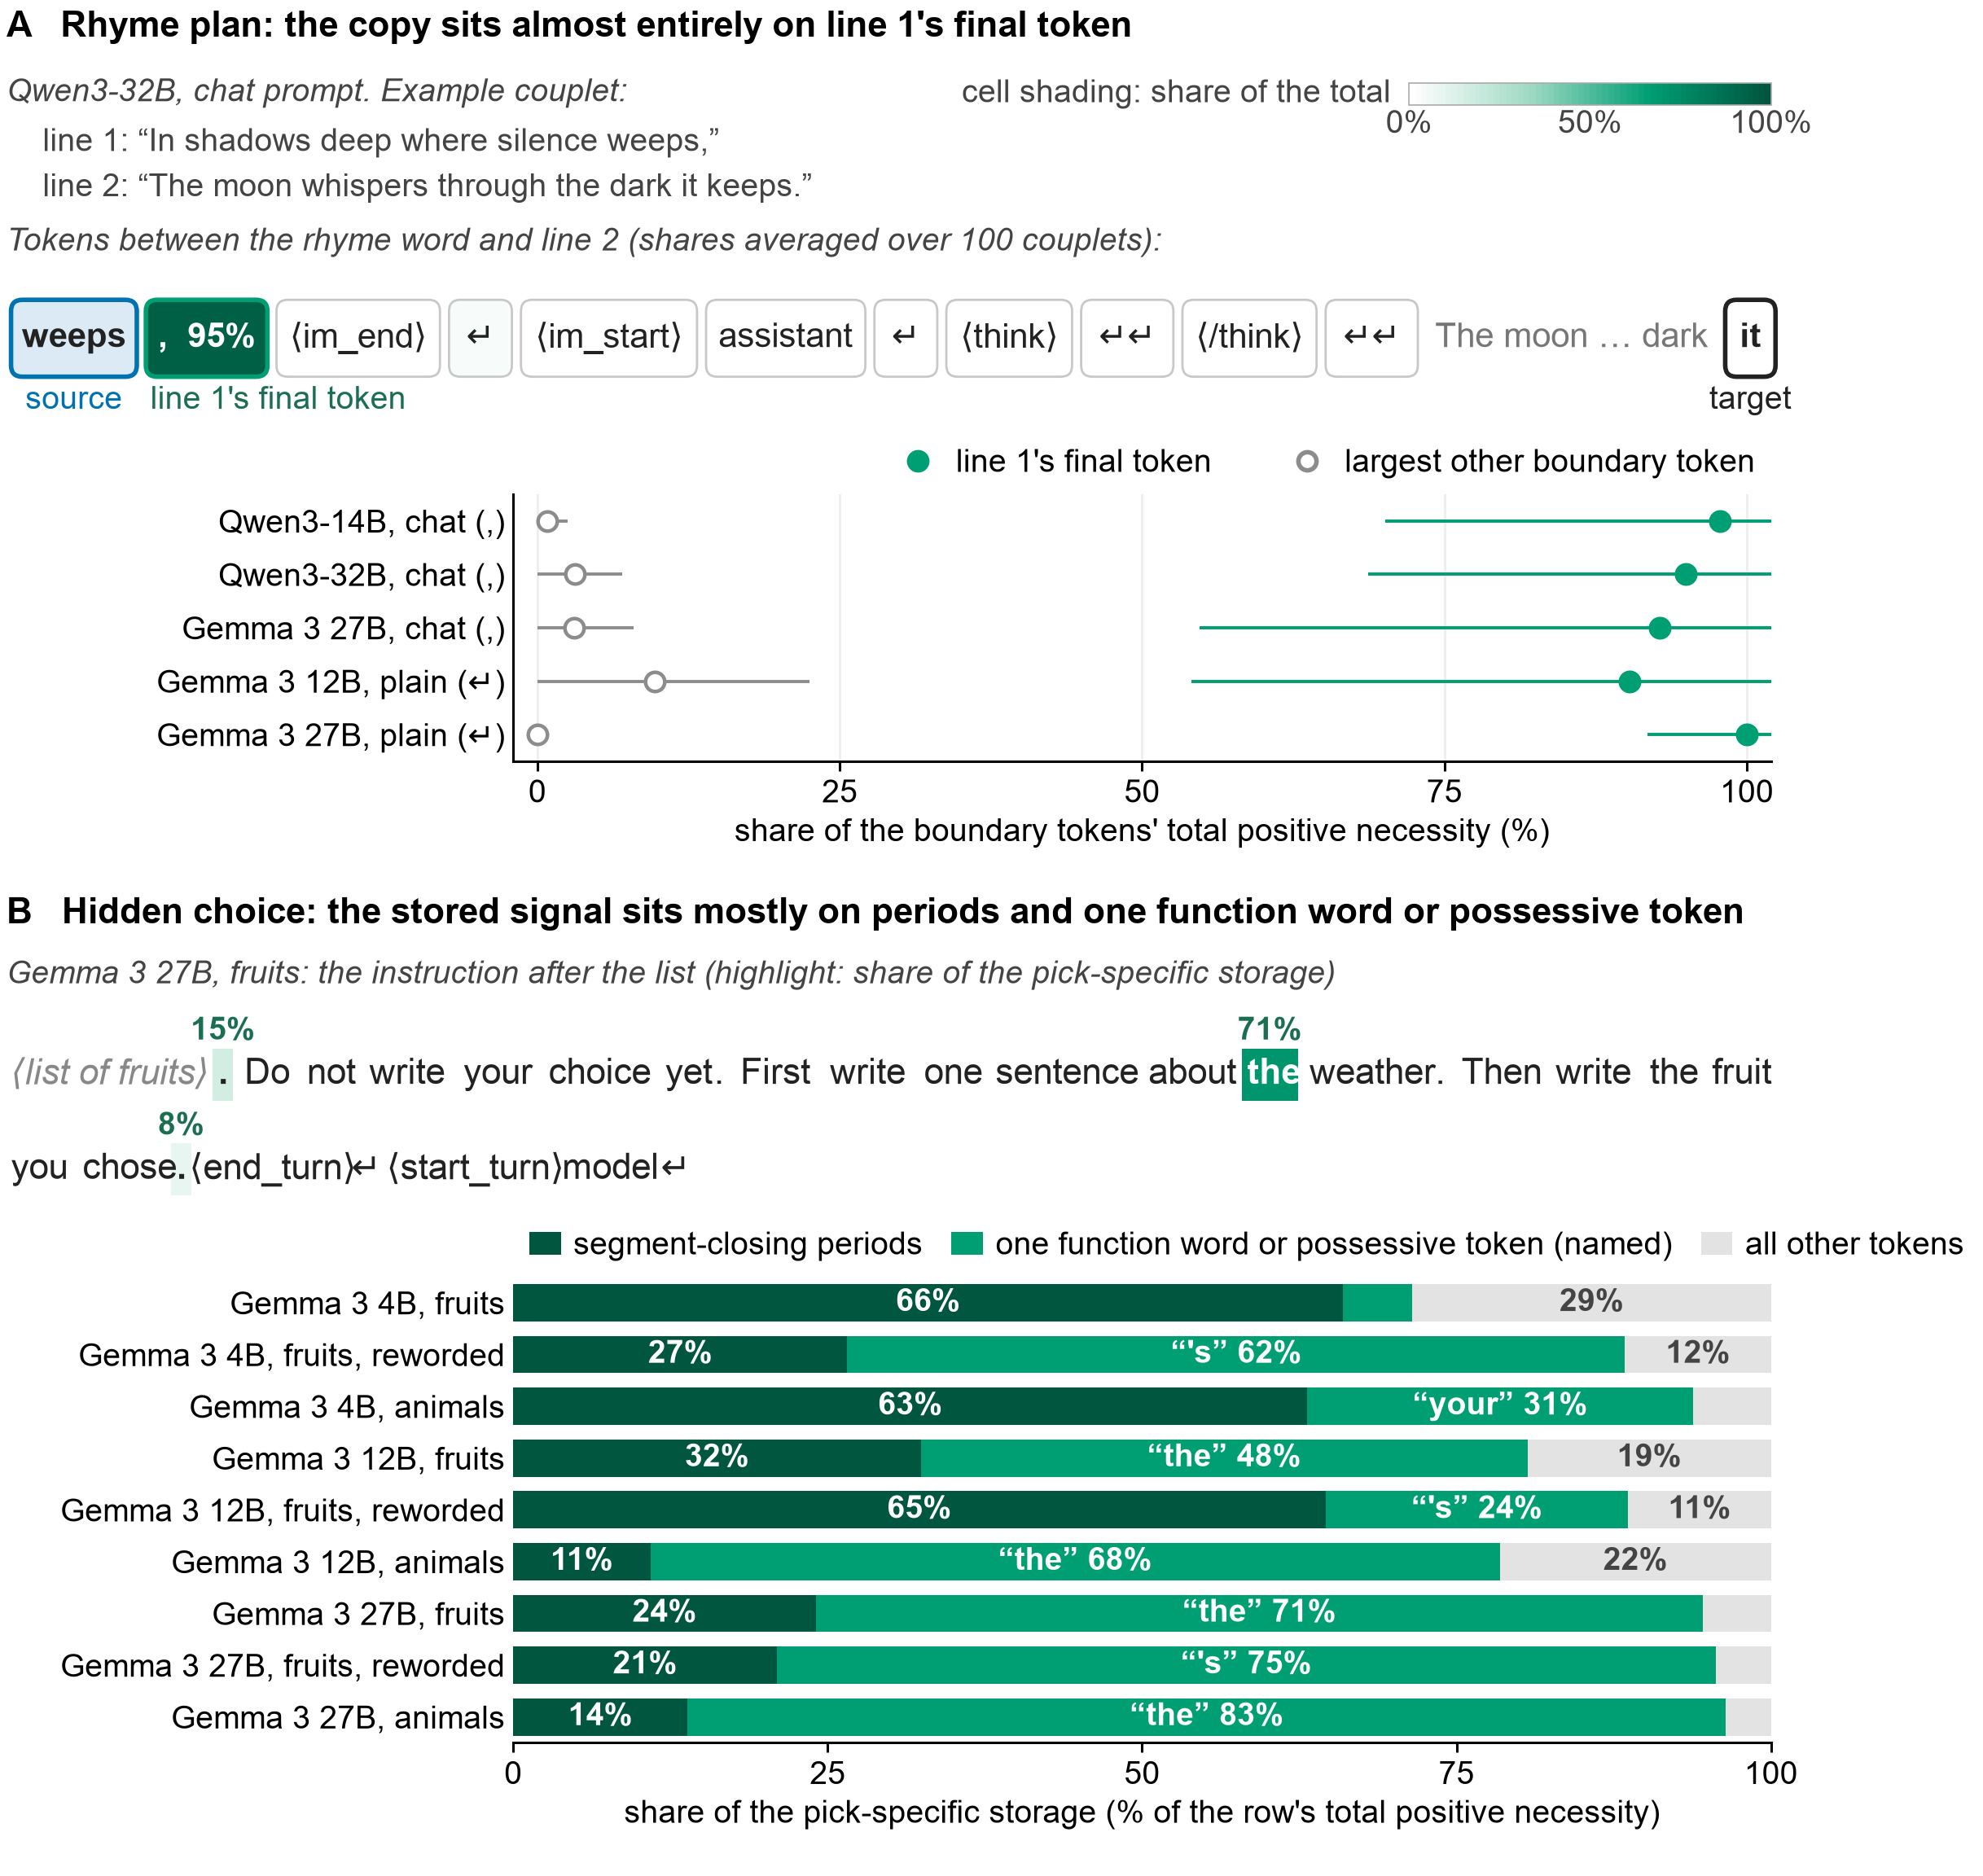
\includegraphics[width=1\linewidth,height=\textheight,keepaspectratio]{manuscript/figures/iclr_fig3_storage_sites.png}

}

\caption{\label{fig-sites}Where stored copies sit. Every value is a
token's \emph{share of necessity}: its interventional necessity (the
loss of the effect when that token alone is reset to its clean state,
with the source edited) divided by the summed positive necessity of all
tokens examined, so the shares of a row add up to 100\%. Cell shading
and printed percentages show the same quantity. \textbf{A:} rhyme plan.
Top, an annotated example (Qwen3-32B, chat prompt): of all tokens
between the rhyme word and line 2, only the comma that ends line 1
matters. Below, for every model with a per-token analysis, the share on
the line's final token (the comma before the chat template, or the
newline in the plain prompt) against the largest share on any other
boundary token. \textbf{B:} hidden choice. The instruction with its
storage tokens highlighted, and for each model and wording the share of
the pick-specific information on the segment-closing periods, on one
function word or possessive token (\emph{the}, \emph{your}, or the
apostrophe of ``today's''), and on all other tokens. At 12B and 27B it
sits mostly on \emph{the} in ``about the weather''; at 4B on the
periods; with the reworded instruction it moves to the list-closing
period and the token before ``weather''. The full token maps are in
Appendix Figure~\ref{fig-storage-all}.}

\end{figure}%

\textbf{The copy appears from about 12 to 14B parameters, and the base
checkpoints we tested have it too.} Table~\ref{tbl-storage} gives the
copy's share of persistence by both measures (bottom row of
Figure~\ref{fig-couplets}).

\begin{itemize}
\tightlist
\item
  In Qwen3 the copy is absent up to 8B (necessity at most 0.9\% of
  persistence in either format). It appears at 14B: 8\% of persistence
  in the chat format and 16\% in the plain format, by necessity. It
  remains at 32B (11\% and 13\%).
\item
  In Gemma 3 it is absent at 1B and 4B, small at 12B (1 to 3\%), and
  present at 27B: 11\% by necessity in the chat format, and in the plain
  format 37\% by sufficiency and 74\% by necessity (\(+19.8\) {[}18.2,
  21.5{]} of \(+26.9\)). The plain format at 27B is the one
  configuration in which more of the plan is read from the line's final
  token than from the rhyme word (19\%): a near-complete hand-off to the
  stored copy, while relay stays at 1\%.
\item
  The base checkpoints store it as well. Qwen3-14B-Base stores 16\% by
  sufficiency, against 13\% for the instruct model in the same format;
  Gemma 3 12B PT stores 5\% and 6\% against 2\% and 3\%. Qwen3-8B-Base,
  like the 8B instruct model, stores nothing. In the three base
  checkpoints tested, the copy is present wherever the matching instruct
  model has it, so it most likely arises in pretraining rather than from
  instruction tuning.
\item
  With same-rhyme donors, the stored copy vanishes (\(-0.02\) to
  \(+0.01\) at 8B to 32B, against \(+0.06\) to \(+1.72\) with
  different-rhyme donors). It encodes the rhyme, not the disruption of
  the edit.
\end{itemize}

\textbf{Where paths interact, the copy matters more than its sufficiency
suggests.} In Gemma 3 27B with the chat prompt, the stored copy alone
moves the rhyme by only \(+0.68\), yet resetting it removes \(+4.87\)
{[}3.18, 6.73{]} of a persistence of \(+43.1\). The additivity gap is
29\% of persistence (Qwen3 at most 5\%). The target combines the rhyme
word and the copy. When only one of them is edited, it reads conflicting
evidence and moves less than the two effects would suggest. This is
redundant storage: a second lookup site that backs up the first.
Reporting sufficiency alone would miss most of it. Shapley values, the
average of the two measures, are given in Appendix
Section~\ref{sec-app-couplets}.

\begin{table}

\caption{\label{tbl-storage}The copy at the line's final token, as a
share of persistence (100 couplets per run). Sufficiency: the boundary
positions alone receive their edited-run states. Necessity: the boundary
positions alone are reset with the rhyme word edited. --: not run.}

\centering{

\footnotesize
\setlength{\tabcolsep}{4pt}
\begin{tabular}{@{}lcccc@{}}
\toprule
Model & Chat: sufficiency & Chat: necessity & Plain: sufficiency & Plain: necessity\\
\midrule
Qwen3-1.7B & 0\% & $-4$\% & 0\% & 1\%\\
Qwen3-4B & 0\% & $-1$\% & 1\% & 0\%\\
Qwen3-8B & 0\% & 0\% & 1\% & 1\%\\
Qwen3-8B-Base & -- & -- & 1\% & 0\%\\
Qwen3-14B & 5\% & 8\% & 13\% & 16\%\\
Qwen3-14B-Base & -- & -- & 16\% & --\\
Qwen3-32B & 8\% & 11\% & 10\% & 13\%\\
Gemma 3 1B & 0\% & 0\% & 1\% & 0\%\\
Gemma 3 4B & 1\% & -- & 0\% & --\\
Gemma 3 12B & 0\% & 1\% & 2\% & 3\%\\
Gemma 3 12B PT & -- & -- & 5\% & 6\%\\
Gemma 3 27B & 2\% & 11\% & 37\% & \textbf{74\%}\\
\bottomrule
\end{tabular}

}

\end{table}%

\textbf{Reconciling published accounts.} Accounts of rhyme planning
disagree on where the plan lives. The disagreement dissolves once both
lookup sites are measured.

\begin{itemize}
\tightlist
\item
  \citet{hanna2026latent} find that attention heads near the end of line
  2 read the rhyme word, and that blocking them sharply reduces rhyming
  at every size up to 14B. In our terms this is direct retrieval
  together with the late lookup, which dominate at every Qwen3 size.
\item
  \citet{lindsey2025biology} find Claude's plan at the newline ending
  line 1, and \citet{maar2026plan} steer successfully at the end of the
  line. This is the stored copy, which appears in larger models.
\item
  \citet{ma2026plan} patch single layers in plain-text couplets. They
  report a hand-off from the rhyme word to the newline in Gemma 3 27B
  only, and none in Qwen3-32B. Our plain-format measurements agree:
  Gemma 3 27B reads more of the plan from the stored copy (37\%) than
  from the rhyme word (19\%). Qwen3-32B keeps a partial copy (10 to
  13\%), which a single-layer patch of the naturally computed state can
  plausibly miss.
\item
  \citet{jacopin2026improvisation} finds no newline effect at 0.6B to
  2.6B. We also find no copy below 8B.
\end{itemize}

Each account is correct for the configuration it studies. The
proportions of the two sites depend on scale, family and prompt format.

\section{Computed and written values}\label{sec-app-computed}

\textbf{Sums.} The prompt poses a two-digit addition. The model writes
an answer-neutral filler of 0 to 32 tokens and then the answer (104
items per model, Qwen3 1.7B to 32B; accuracy 95 to 100\%). The committed
design named the question mark as the position where the sum would be
computed. Donor states there move the answer by \(-0.08\) to \(+0.07\)
log-odds, so the efficacy gate fails at every size. That shows only that
the question mark does not hold the sum. The stronger test edits every
position from the question mark to the answer together: this block moves
the answer by at most 6.4\% of the effect of donor operand digits
(\(+17\) to \(+54\); 6.4\% at 32B, \(+1.10\) {[}0.93, 1.27{]} of
\(+17.2\), and at most 3.4\% at the smaller sizes). The downstream block
is small beside the operand edit, which is consistent with the answer
re-reading the visible operands; recomputation itself was not measured.

\textbf{Variable chains.} Sums are cheap to recompute. A chain of
updates (\texttt{a\ =\ 23}, \texttt{b\ =\ a\ +\ 4},
\texttt{c\ =\ b\ +\ 7}, \ldots, \texttt{What\ is\ e?}) makes
recomputation at the answer costly and makes an indirect path the
natural one. The running value could be passed from statement to
statement, so this task was designed as a second positive-control
candidate for an indirect path. It is not one. Donor states at the
starting value's digits move the answer strongly (at 14B: \(+30.9\),
\(+18.5\) and \(+6.4\) for \(K=1,3,5\) updates). Where single positions
were edited (1.7B to 14B; at 32B only the block was run), donor states
at any later position, or at any statement end, move it by less than 0.4
in absolute value. Donor states at \emph{every} position after the
starting value together, a test that would detect a running value stored
redundantly, move it by at most 4.9\% of the source-digit effect (32B,
\(K=1\): \(+0.81\) {[}0.61, 1.03{]} of \(+16.5\)). The other cell whose
interval excludes zero is 14B at \(K=3\) (\(+0.44\) {[}0.08, 0.82{]} of
\(+18.5\), 2.4\%). At 32B the block is \(-0.02\) {[}\(-0.33\), 0.29{]}
of \(+10.1\) at \(K=3\) and \(-0.00\) {[}\(-0.22\), 0.19{]} of \(+5.2\)
at \(K=5\). In the remaining size and length combinations the interval
includes zero. Figure~\ref{fig-computed} shows the \(K=3\) series, which
stays near zero. The downstream block is small beside the source edit,
which is consistent with the answer re-reading the chain. Accuracy is
consistent with recomputation at the answer. It falls steeply with chain
length, from 97 to 100\% at \(K=1\) to 1 to 17\% at \(K=5\) (Appendix
Figure~\ref{fig-computed-extra}). At \(K=5\), where maintaining a
running value would make more answers correct, the downstream block's
interval includes zero at every size. That agreement is correlational,
not a test of what the model could do.

\begin{figure}

\centering{

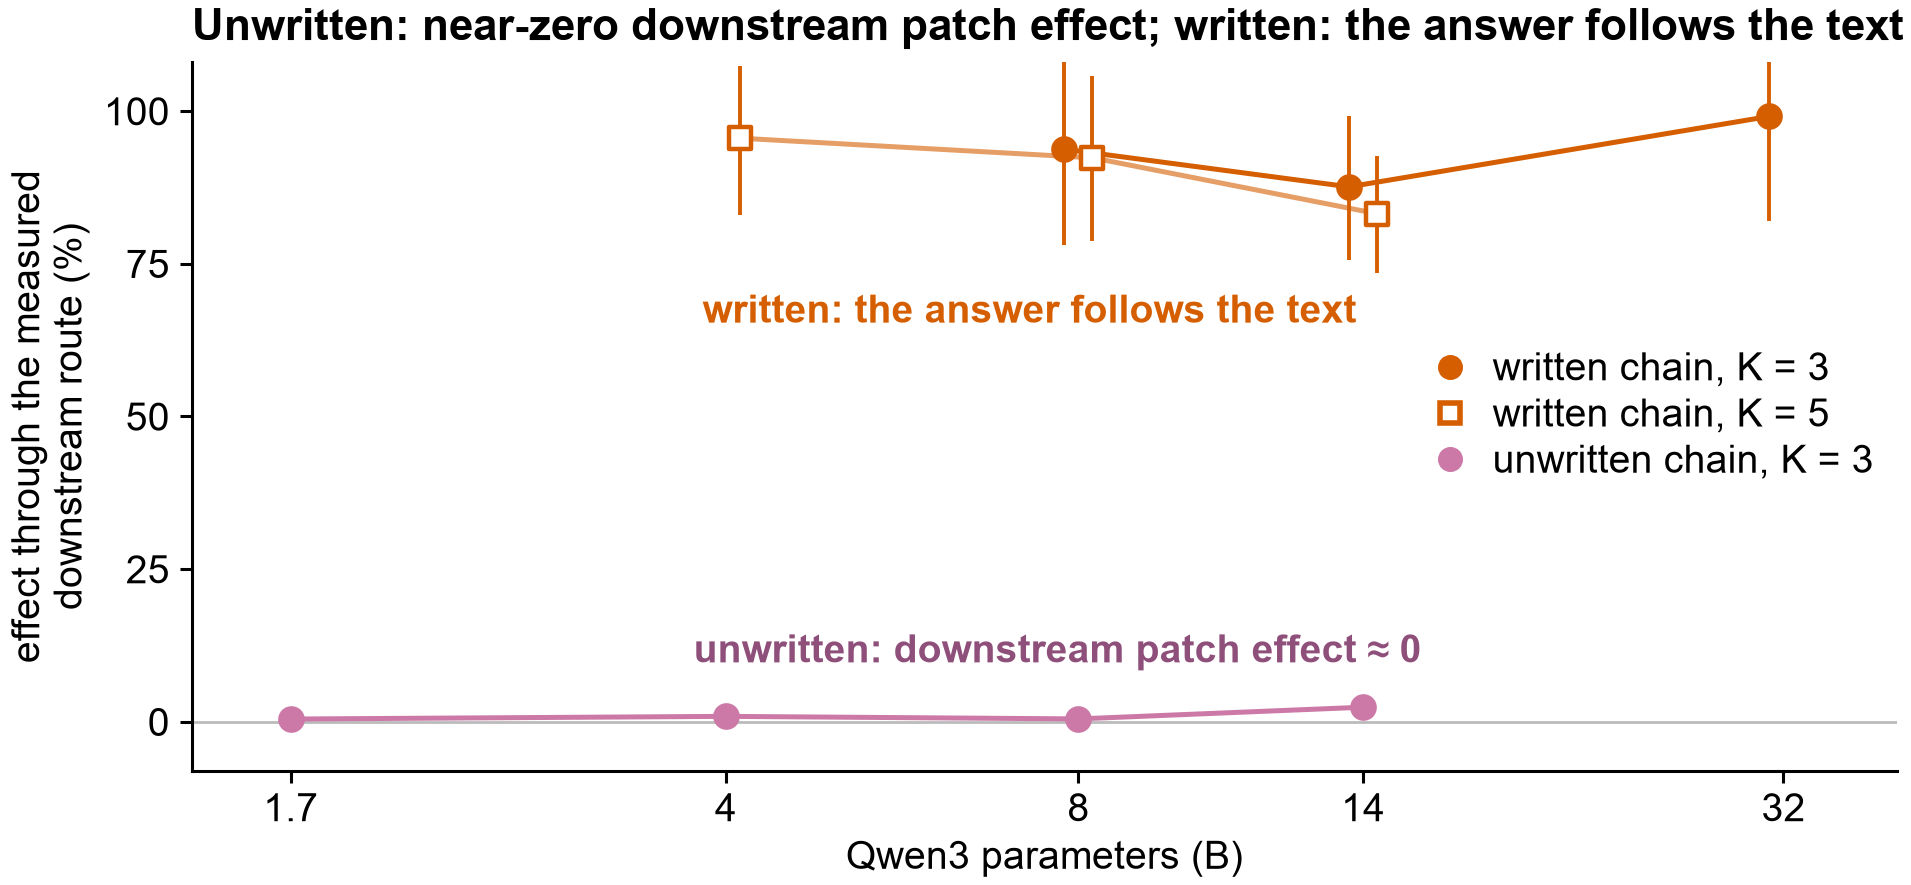
\includegraphics[width=1\linewidth,height=\textheight,keepaspectratio]{manuscript/figures/iclr_fig5_computed_and_written.png}

}

\caption{\label{fig-computed}Unwritten versus written computed values
(Qwen3 variable chains), on one axis with two denominators.
\emph{Unwritten:} the effect of donor states at every position after the
source, as a share of the effect of editing the source digits.
\emph{Written:} emission divided by the total effect. 95\% intervals.
For unwritten chains (\(K=3\) updates) this downstream patch effect
stays near zero, which is consistent with the answer re-reading the
source; recomputation itself is not measured. \emph{Written}: the share
that goes through the values the model writes (emission; \(K=3\) and
\(K=5\)); the answer follows the text. The remainder of the written case
is the bypass to the edited source. The two series cover different sizes
because of which runs exist: both series now cover 1.7B to 32B; at 32B
the unwritten point comes from the block edit alone.}

\end{figure}%

\textbf{In these chains the answer follows the written values.} We
return to the variable chains of Section~\ref{sec-computed}, now with
the instruction ``Compute each variable in order, one per line, then
state the value of \(e\)''. The model writes each intermediate value.
The edit at the starting value's digits makes it write the donor's
values in 86 to 100\% of items. We cut the written chain after the
second-to-last value and measure the answer's first digit. The six-cell
split then shows how much of the effect goes through the written values
(emission) and how much bypasses them (persistence with the text fixed).

\begin{itemize}
\tightlist
\item
  Emission accounts for 92\% and 96\% of the effect at 1.7B (\(K=3\) and
  \(K=5\)), 93\% and 96\% at 4B (\(K=3\) and \(K=5\)), 94\% and 92\% at
  8B, 88\% and 83\% at 14B, and 98\% and 101\% at 32B (every chain
  usable after the parser fix).
\item
  The bypass, which re-reads the edited source digits, is 4 to 8\% at 4B
  and 8B and 12 to 17\% at 14B. At 32B it is \(+0.15\) {[}0.03, 0.28{]}
  (2\%) at \(K=3\) and \(-0.08\) {[}\(-0.17\), 0.01{]} at \(K=5\). At
  32B and \(K=5\), emission is 101\% of the total because that bypass is
  negative. Emission plus the bypass equals the total (\(+6.62\) and
  \(-0.08\) sum to \(+6.54\)).
\end{itemize}

Written reasoning is not decorative in these models. The answer follows
the written values, and the part that re-reads the source stays below
17\% at every size tested. The couplets give the same picture on a
smaller scale: the emitted line-2 words account for 13 to 25\% of the
rhyme effect (Section~\ref{sec-couplets}).

\textbf{Leverage.} How much of an effect goes through a written token
depends on how much that token matters. For a binary mediator
\(B\in\{b_0,b_1\}\), such as the article \emph{a} or \emph{an} before a
planned noun, let \(q_i=P(B=b_1\mid I=i)\) be the probability of writing
\(b_1\) with the intervention off (\(i=0\)) or on (\(i=1\)). Let
\(Y(0,b)\) be a scalar outcome, here \(\log p(\text{planned noun})\),
with the intervention off and the mediator fixed to \(b\).
Policy-weighted emission is defined as
\(E_{\rm emit}=\sum_b [q_1(b)-q_0(b)]\,Y(0,b)\) (Appendix
Section~\ref{sec-app-sixcell}). For a binary mediator it equals, by
definition,

\[
E_{\rm emit} \;=\; (q_1-q_0)\,\big(Y(0,b_1)-Y(0,b_0)\big).
\]

This is the change in the policy-weighted expected outcome, not the
change in the logarithm of the marginal probability. The effect through
the text is the change in what is written, times how much the written
token matters to what follows. We call the second factor the token's
\emph{leverage}. We apply the six-cell assay to the a/an planning
features of \citet{hanna2026latent}, which are selected by a rule with
no article criterion. We use their per-layer transcoders for Qwen3 0.6B,
1.7B and 4B and reproduce their node counts exactly on 297 to 344 of 349
prompts.

\begin{itemize}
\tightlist
\item
  At 4B, where they report planning, the features have a bidirectional,
  feature-specific effect on the planned noun. Of that effect, 92 to
  94\% travels through the generated article. The effect that bypasses
  the article (\(+0.012\) {[}0.000, 0.024{]} for amplified features) is
  at the level of randomly chosen features (\(-0.003\) {[}\(-0.019\),
  0.013{]}).
\item
  Stratified by leverage (Appendix Figure~\ref{fig-computed-extra}), the
  effect through the article scales with leverage, while the effect
  bypassing it stays small and constant. The article accounts for 53 to
  82\% of the effect in the lowest-leverage tertile and 94 to 96\%
  elsewhere.
\item
  The product of policy movement and leverage predicts the effect
  through the article better than policy movement alone (correlation
  0.886 against 0.831 for amplified features).
\item
  At 0.6B and 1.7B the effects are small and travel almost entirely
  through the article.
\end{itemize}

\begin{figure}

\centering{

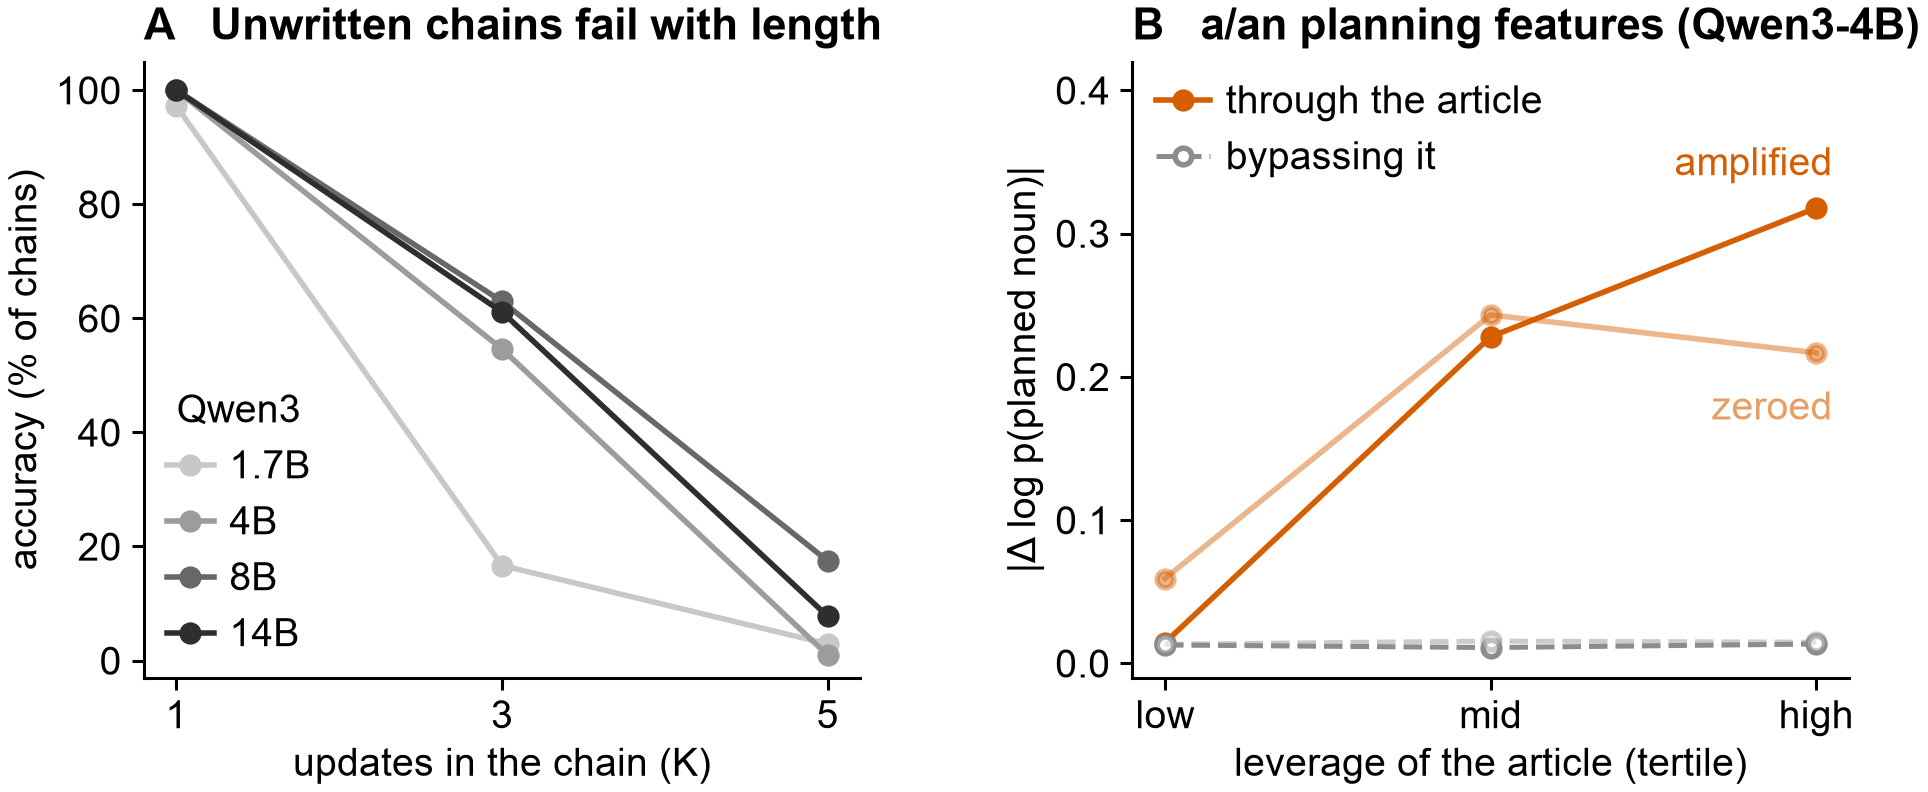
\includegraphics[width=1\linewidth,height=\textheight,keepaspectratio]{manuscript/figures/iclr_figA_computed_extra.png}

}

\caption{\label{fig-computed-extra}Computed values, supporting panels.
\textbf{Left:} accuracy of unwritten variable chains (Qwen3 1.7B to 14B)
against the number of updates. \textbf{Right:} a/an planning features in
Qwen3-4B. The effect on the planned noun through the article
(vermillion) against the effect bypassing it (grey), by tertile of the
article's leverage over the planned noun, for amplified and zeroed
features.}

\end{figure}%

\textbf{Sum prompts.} The user turn is
\texttt{/no\_think\ What\ is\ \{a\}\ +\ \{b\}?}. The assistant turn is
prefilled with the filler and \texttt{The\ answer\ is}. The target is
the first digit of the answer. Table~\ref{tbl-sums} gives the efficacy
scan.

\begin{table}

\caption{\label{tbl-sums}Sums: donor states at each position group
(log-odds toward the donor's first digit; 104 items).}

\centering{

\footnotesize
\setlength{\tabcolsep}{4pt}
\begin{tabular}{@{}lccccc@{}}
\toprule
 & 1.7B & 4B & 8B & 14B & 32B\\
\midrule
Accuracy (all filler lengths) & 95--100\% & 100\% & 100\% & 100\% & 100\%\\
Donor state at \texttt{?} (committed) & $+0.07$ & $+0.01$ & $-0.08$ & $-0.06$ & $-0.03$\\
Every position from \texttt{?} to the target & $+0.30$ & $+0.58$ & $-0.12$ & $+1.62$ & $+1.10$\\
Operand digits & $+47.8$ & $+48.0$ & $+53.6$ & $+47.3$ & $+17.2$\\
\bottomrule
\end{tabular}

}

\end{table}%

\textbf{Chain prompts.} The user turn is
\texttt{a\ =\ \{v0\}\textbackslash{}nb\ =\ a\ +\ \{d1\}\textbackslash{}n...\textbackslash{}nWhat\ is\ \{last\}?},
with \(K=1,3,5\) updates, 103 to 108 items per \(K\), and the same
increments for original and donor, so the tokens align.
Table~\ref{tbl-chains} gives the edits.

\begin{table}

\caption{\label{tbl-chains}Variable chains (unwritten). Donor states at
the starting value's digits versus at every later position (the block
edit), \(K=1/3/5\).}

\centering{

\footnotesize
\setlength{\tabcolsep}{4pt}
\begin{tabular}{@{}llll@{}}
\toprule
 & Accuracy & Source digits & Every later position\\
\midrule
Qwen3-1.7B & 97 / 17 / 3\% & $+36.3$ / $+24.4$ / $+13.6$ & $-0.02$ / $+0.11$ / $+0.04$\\
Qwen3-4B & 100 / 55 / 1\% & $+47.1$ / $+32.2$ / $+20.1$ & $-0.07$ / $+0.29$ / $-0.20$\\
Qwen3-8B & 100 / 63 / 17\% & $+45.1$ / $+31.1$ / $+18.4$ & $+0.05$ / $+0.15$ / $-0.07$\\
Qwen3-14B & 100 / 61 / 8\% & $+30.9$ / $+18.5$ / $+6.4$ & $+0.09$ / $+0.44$ / $+0.22$\\
\bottomrule
\end{tabular}

}

\end{table}%

\section{Per-token storage maps}\label{sec-app-storage}

\begin{figure}[H]

\centering{

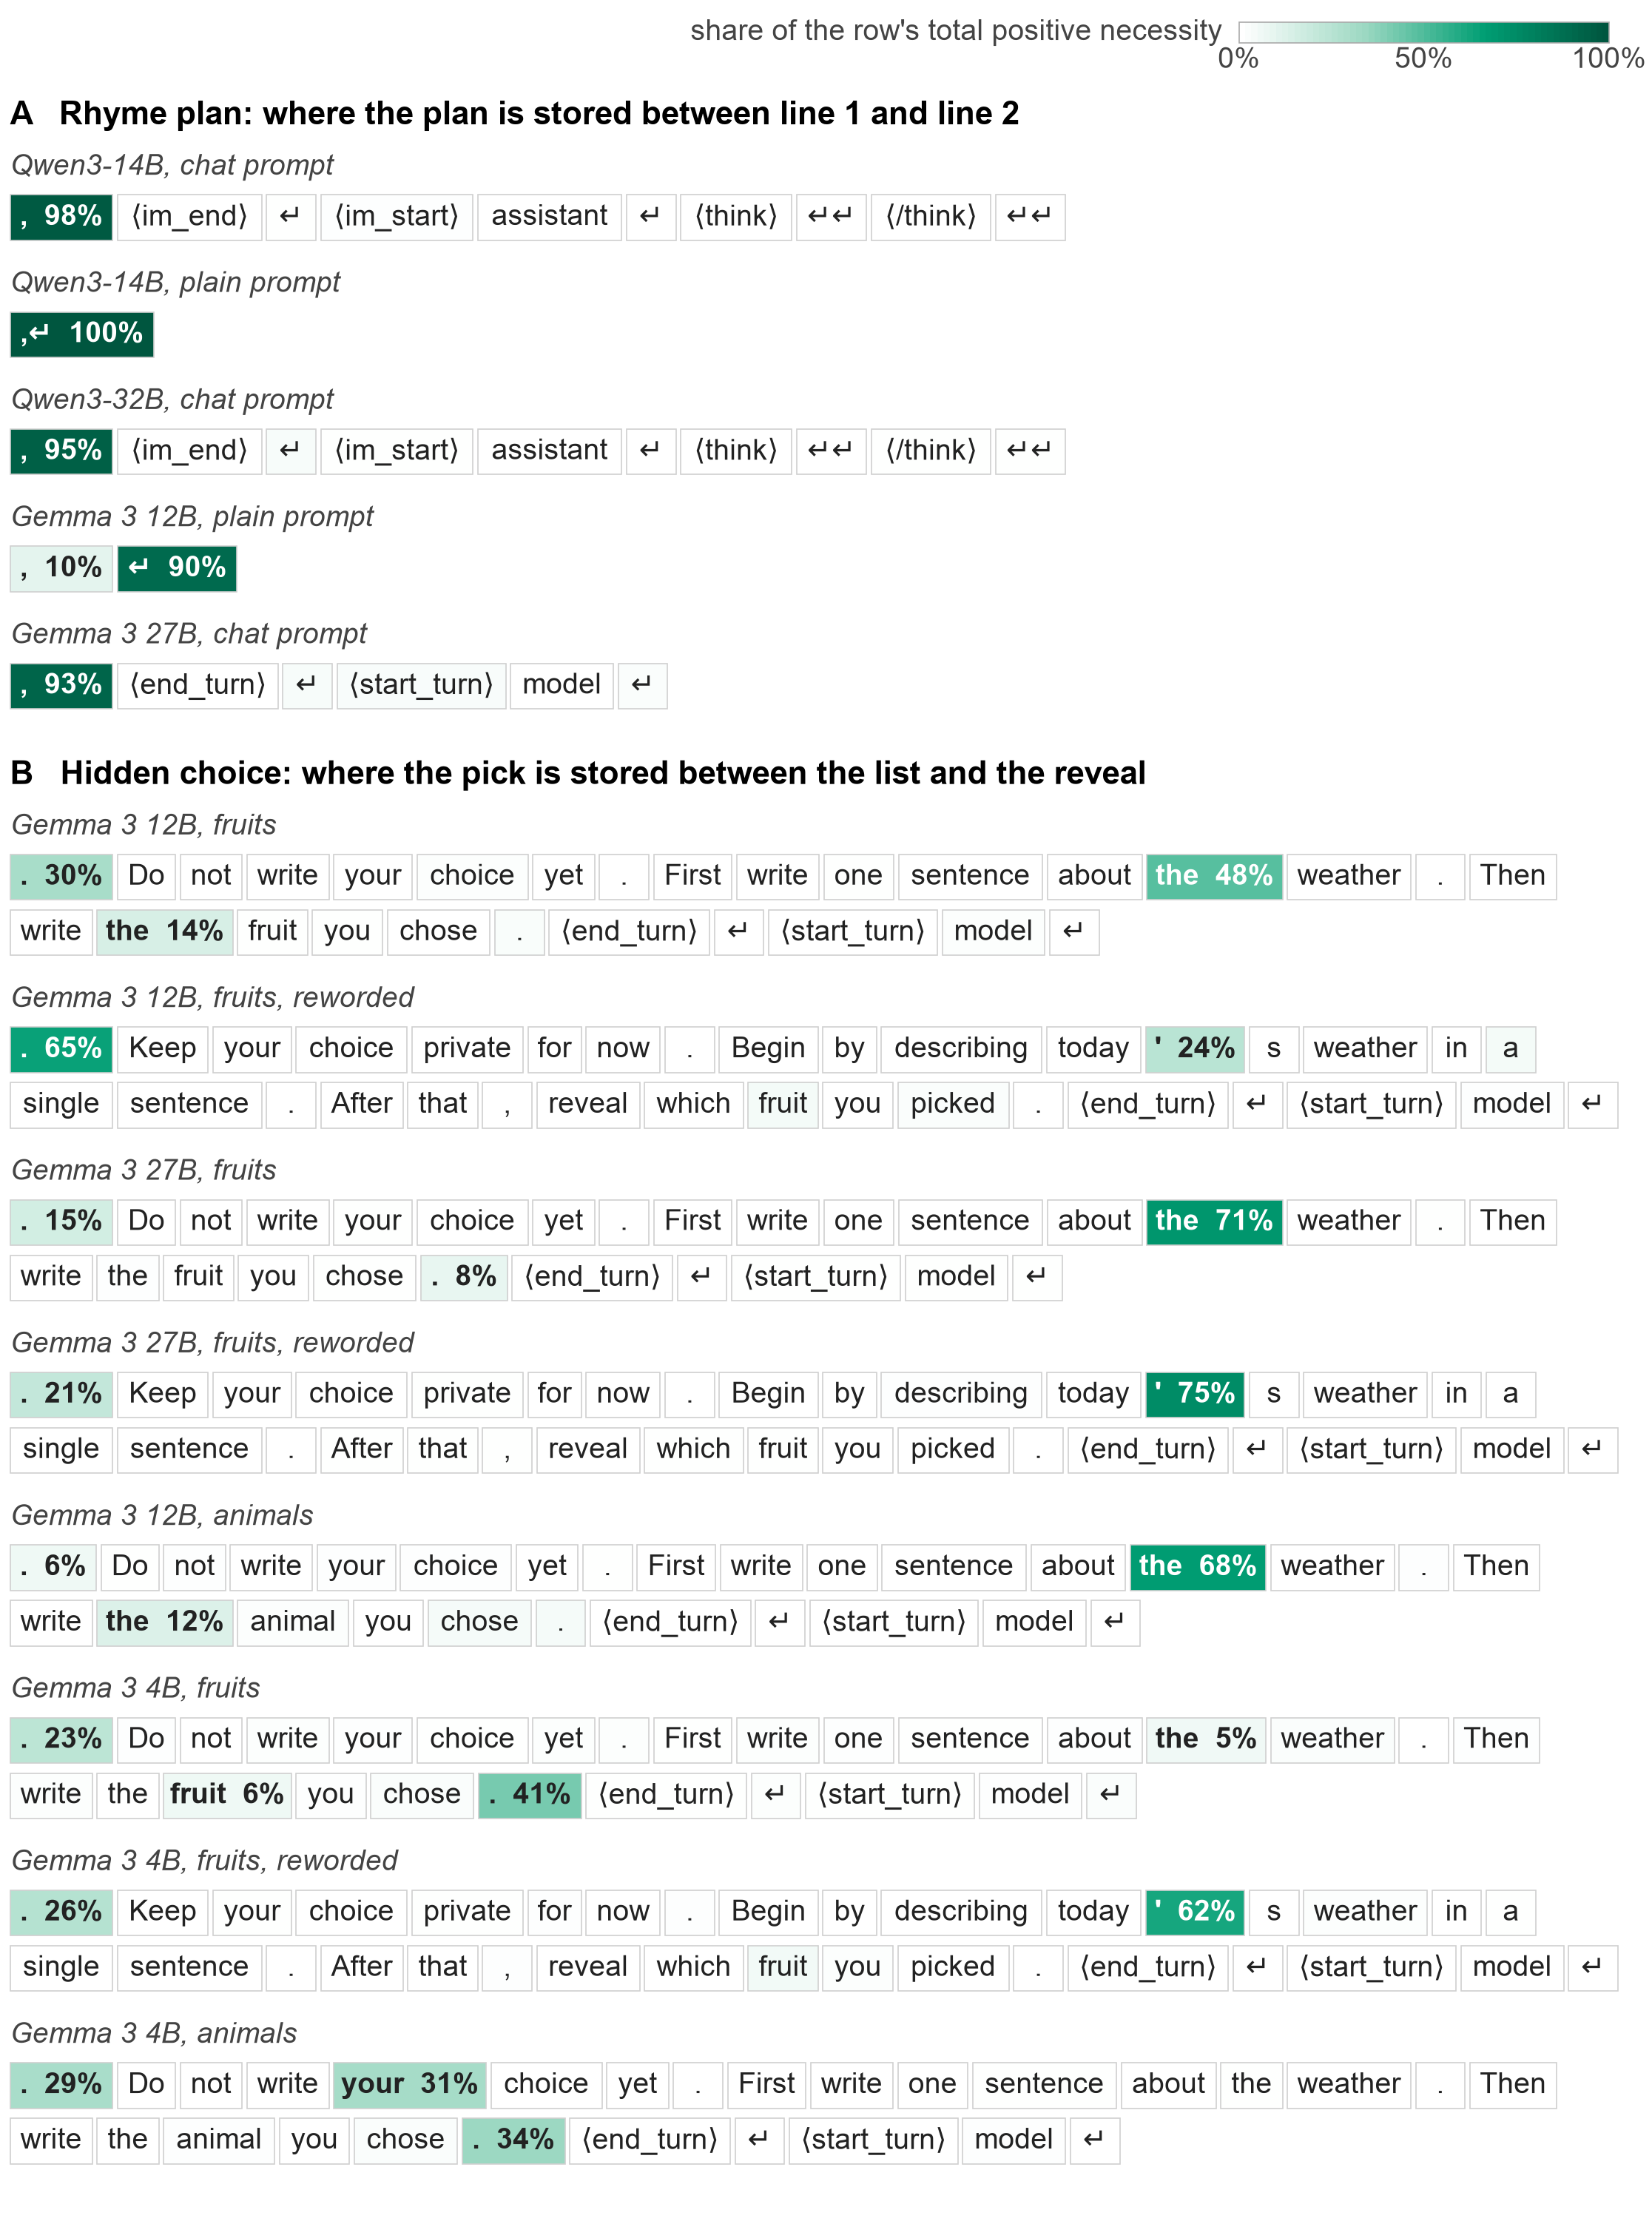
\includegraphics[width=1\linewidth,height=\textheight,keepaspectratio]{manuscript/figures/iclr_figA_storage_all.png}

}

\caption{\label{fig-storage-all}Per-token necessity for every model and
wording analysed. Each cell is one token; the shade and the printed
value give its share of necessity (Figure~\ref{fig-sites}): the loss of
the effect when that token alone is reset to its clean state, with the
source edited, as a share of the row's summed positive necessity. Top
rows: tokens between the rhyme word and line 2. Bottom rows: tokens
between the hidden-choice list and the reveal (pick-specific part).}

\end{figure}%

\section{Settings built to favour relay: details}\label{sec-app-stress}

\subsection{Beyond the attention window}\label{sec-app-distance}

Gemma 3 alternates five local layers with a 1,024-token sliding window
\citep{beltagy2020longformer} with one global layer \citep{gemma3}. Once
line 1 lies more than 1,024 tokens before the rhyme position, five of
six layers can no longer read it. We insert \(D\) tokens of neutral
filler, a seeded arrangement of fixed everyday sentences, at the start
of the model's turn, followed by a fixed cue (\texttt{Next\ line:}). The
model then writes line 2. The indirect path is split into three groups
of intermediate positions: the stored copy (the prompt positions after
line 1), the filler, and the generated text (the cue and line 2). The
committed decision number is the share of persistence that takes the
indirect path through the generated text: ``go'' at 25\% or more,
``stop'' below 10\%, and extension to 50 couplets in between. A
full-attention control, Qwen3-14B, showed before the Gemma result that
indirect \emph{shares} can rise with distance only because direct
retrieval weakens. We therefore added, before that result, the rule that
a rise counts only if the absolute indirect effect also grows.

Table~\ref{tbl-distance} gives the extended run. At 2,000 tokens, Gemma
3 27B still writes a rhyming line 2 in 82\% of couplets, but persistence
falls from \(+42.4\) to \(+26.4\). The model reads less of the plan from
the rhyme word: direct retrieval falls from 66\% to 40\% of persistence.
It relies instead on the stored copy at the line's final token, which is
necessary for \(+13.0\) {[}10.0, 16.1{]}, about half of persistence. The
absolute indirect effect grows about thirteenfold (\(+1.0\) to
\(+13.1\)), mostly through the stored copy. The filler passes on nothing
(\(+0.3\) by sufficiency, \(+0.15\) by necessity). The indirect path
through the generated text rises from about 1\% to 12\% by sufficiency
(\(+3.2\) {[}2.2, 4.3{]}); its necessity is \(+2.7\), or 10\%. This
block contains the cue and all of line 2, including its last three
positions, so it mixes relay with the late lookup; the split was not
run. It is the largest generated-text block we measure, a borderline
case rather than a demonstrated exception: by the committed rule it
falls between ``stop'' and ``go'', and how much of it is relay remains
unresolved. Even at 2,000 tokens it is a minority path, about an eighth
of the effect.

The window curve, committed before its result, predicted a change
specifically between 1,000 and 1,500 tokens. The interior distances use
18 couplets each and the endpoints the 50 couplets of
Table~\ref{tbl-distance}, so the curve is not one uniform sample. It is
only partly supported. Direct retrieval is 66\%, 64\%, 54\%, 40\% and
40\% of persistence at 0, 500, 1,000, 1,500 and 2,000 tokens, and the
stored copy is necessary for 11\%, 25\%, 30\%, 45\% and 49\%. The
largest point-estimate step is where line 1 leaves the window, but the
shift has begun at 500 tokens, inside it. The indirect path through the
generated text is 11\%, 9\%, 13\% and 12\% by sufficiency at the four
nonzero distances (by necessity 10\%, 14\%, 11\% and 10\%): it appears
once filler is present and does not grow with distance. We therefore
describe a long-distance shift toward the stored copy, steepest across
the window, rather than a precisely located window-edge transition.

\begin{table}

\caption{\label{tbl-distance}Indirect paths at a distance, Gemma 3 27B
(chat prompt; 50 couplets per distance; 95\% intervals). Shares are of
persistence at the same distance. The generated-text block is the cue
plus all of line 2; it is not split into late lookup and relay.}

\centering{

\small
\setlength{\tabcolsep}{4pt}
\begin{tabular}{@{}lll@{}}
\toprule
 & $D=0$ & $D=2{,}000$\\
\midrule
line 2 rhymes with line 1 & 98\% & 82\%\\
persistence & $+42.4$ [38.6, 46.0] & $+26.4$ [23.8, 28.9]\\
direct retrieval & $+28.0$ (66\%) & $+10.5$ (40\%)\\
stored copy: sufficiency / necessity & $+0.1$ / $+4.6$ (11\%) & $+9.7$ / \textbf{$+13.0$} (49\%)\\
filler: sufficiency / necessity & 0.0 / 0.0 & $+0.3$ / $+0.15$ [$-0.26$, 0.57]\\
generated text: sufficiency / necessity & $+0.5$ / $+7.3$ & \textbf{$+3.2$} (12\%) / $+2.7$ (10\%)\\
\bottomrule
\end{tabular}

}

\end{table}%

Three further models show what happens when lookup gets harder without a
strong stored copy. They also separate distance from the window.

\begin{itemize}
\tightlist
\item
  \emph{Gemma 3 12B}, which keeps only a small stored copy
  (Table~\ref{tbl-storage}), loses the plan. The window curve, committed
  before its result, predicted that the plan would survive while line 1
  is inside the window (500 and 1,000 tokens) and vanish outside it.
  Instead, the plan fades gradually and is mostly gone inside the
  window. Second lines rhyme in 100\%, 39\%, 8\%, 0\% and 0\% of
  couplets at 0, 500, 1,000, 1,500 and 2,000 tokens, and persistence
  falls from \(+40.5\) to \(+11.5\) {[}8.1, 14.9{]} at 500 tokens and
  \(+4.0\) at 1,000. At 12B the loss reflects the distance itself, not
  the window. No indirect path takes over: the absolute indirect effect
  stays at \(+0.8\) to \(+2.3\), and relay at or below \(+0.9\).
\item
  \emph{Qwen3.5-9B}, a hybrid whose attention layers have no window,
  also fades: rhyming falls from 92\% to 4\% at 2,000 tokens. What
  remains of persistence (\(+3.6\)) is still 81\% direct retrieval, and
  the absolute indirect effect does not grow (\(+1.2\) to \(+0.8\)).
\item
  \emph{Qwen3-14B}, with full attention, largely abandons the task after
  the filler (8\% rhyming), and its absolute indirect effect stays flat
  (\(+2.3\) to \(+2.8\)).
\end{itemize}

Across the four models, distance moves reliance onto a stored copy where
one exists, and otherwise costs the plan. In no model does an indirect
path through the generated text take over. The 12\% in Gemma 3 27B is
the unsplit generated-text block, including its last three positions.
The rhyme word and the line's final token lie at the same distance from
the target, yet the global layers of Gemma 3 27B read the line's final
token. This fits the view of separator tokens \citep{chen2024sepllm} and
label words \citep{wang2023labelwords} as summaries of their segment.

\subsection{Recurrent memory}\label{sec-app-recurrent}

Qwen3.5 \citep{qwen2026qwen35} interleaves three Gated DeltaNet layers
\citep{yang2025gateddeltanet} with each full-attention layer. A
recurrent layer holds a fixed-size state that is updated position by
position. In those layers, information from the source can reach a later
position only through that state, passed along every intervening
position by construction and invisible in the text. The attention layers
can still look it up. The test therefore asks which path the model uses
when both are available. We split persistence by layer type. In the
\emph{attention-only} cell, the donor state enters at the source, but
the input of every recurrent layer at the source is restored to its
clean value, so the edit can move forward only through the attention
layers. The \emph{recurrent-only} cell is the converse. A cell with both
layer types blocked is a sanity check. The rule committed in advance was
``go'' if recurrent-only is at least 25\% of persistence with its
interval above zero, and ``stop'' if it is below 10\%. It is decided on
the largest model; smaller sizes give the trend.

When the donor signal can enter at the source through either layer type,
entry through the attention layers accounts for nearly all of its
effect. At 4B and 9B (40 couplets each), the recurrent-only cell is
\(+0.28\) {[}0.07, 0.49{]} and \(+0.55\) {[}0.31, 0.79{]}: 3\% and 4\%
of persistence. The attention-only cell accounts for 97\% and 96\%. At
the decisive size, 27B (48 recurrent and 16 attention layers; 24
couplets), recurrent-only is \(+0.41\) {[}0.18, 0.64{]}, 2\% of
persistence \(+18.8\) {[}16.3, 21.3{]}, and attention-only 95\%. As a
sanity check, blocking both layer types at the source cancels the donor:
that cell is zero on every couplet, as it must be. Decision: stop.
Although three quarters of the layers can pass the plan forward only
through the recurrent state, a donor signal that enters through them at
the source produces only 2 to 4\% of persistence. The design controls
which layer type receives the donor signal at the source; it does not
isolate every later path through each layer type, so it measures the
share of donor entry, not the recurrent memory's natural share. Entry
through the recurrent layers is small but nonzero, which bounds the
principle at 2 to 4\% of persistence for this architecture.

\section{Hidden choice}\label{sec-app-hidden}

In every task so far, the content is visible: a reader of the text could
recover the rhyme sound from line 1, or the value from the operands. The
case monitoring cares about is content that cannot be recovered from the
text. We create it with a secret choice. The prompt reads: ``Secretly
choose one fruit from this list: \{4 fruits\}. Do not write your choice
yet. First write one sentence about the weather. Then write the fruit
you chose.'' Under greedy decoding the pick is a deterministic function
of the prompt. It depends on the model's own preferences and on the list
order, so no reader can compute it. For the path split, the model's turn
is prefilled with a fixed weather sentence and ``The fruit I chose is''.
The outcome is the log-odds of the donor's pick against the original
pick at the next token.

\textbf{A small part of the pick-specific signal is stored after the
list, and almost none passes through the sentence.} The donor is the
same list in another order, chosen so that the greedy pick differs. The
reference is a \emph{text swap}: the donor order written into the
prompt, which moves the pick by construction. In Qwen3-8B, Gemma 3 12B
and Gemma 3 27B (100 pairs each), donor states at the prompt positions
after the list move the reveal by 12\%, 15\% and 16\% of the text swap.
The reveal reads all of it directly: the direct-retrieval cell equals
the post-list effect. The part of this stored signal that passes through
the sentence is \(+0.00\) {[}\(-0.04\), 0.05{]}, \(-0.06\) {[}\(-0.14\),
0.01{]} and \(-0.01\) {[}\(-0.10\), 0.08{]}; it is also zero within its
interval in Qwen3-4B and Qwen3-14B. The rest of the pick, 84 to 88\%, is
not reproduced by the post-list patch; it is presumably re-derived at
the reveal from the visible list. The two largest Qwen models are the
exception.

\begin{itemize}
\tightlist
\item
  In \emph{Qwen3-32B}, the indirect path through the sentence is small
  but nonzero: \(+0.06\) {[}0.04, 0.09{]}. That is 2\% of the text swap
  but one eighth of the stored part.
\item
  In the recurrent hybrid \emph{Qwen3.5-27B}, the part of the stored
  signal that passes through the sentence is \(+0.03\) {[}0.02, 0.04{]}:
  1\% of the text swap and one sixth of the stored part. Its sentence
  positions themselves account for 7\% of the text swap (\(+0.15\)
  {[}0.12, 0.18{]}); Qwen3.5-9B gives the same pattern (through the
  sentence 2\%, sentence positions 8\%). These are the largest in any
  model; Qwen3-4B has 5\% and every other model at most 1\%. This is
  expected when every position's recurrent state summarizes the prefix,
  including the list.
\end{itemize}

\textbf{What the stored signal could be.} An order swap cannot separate
a stored pick from a stored copy of the list order. In the out-of-list
control, the donor list shares no item with the original, so the donor's
pick does not occur in the prompt at all. The committed criterion is
that post-list donor states raise the absent pick, and it holds in every
model. After the first results we identified a confound: the positions
might hold a copy of the donor's list rather than its pick. We therefore
added, post hoc, \emph{pick specificity}: the effect on the donor's pick
minus the mean effect on the donor's other items. We then committed it,
before the results, as the primary measure of a replication in a second
domain (animals; disjoint lists of six). The replication confirms that
pick-specific information is stored after the list, in both families
(Figure~\ref{fig-stress} C; Table~\ref{tbl-hidden}). A same-pick null,
committed before its result, gives the converse check. The donor is the
same list in another order with the \emph{same} pick. Post-list donor
states then leave the relative preference for the pick unchanged on
average in Gemma 3 12B: \(-0.19\) {[}\(-0.53\), 0.16{]}, against
\(+1.01\) {[}0.78, 1.24{]} with out-of-list donors. Gemma 3 27B gives
the same null: \(-0.42\) {[}\(-0.96\), 0.10{]}, against \(+2.48\) with
out-of-list donors.

These controls do not settle what the stored information is. The
post-list positions could hold the pick itself. They could also hold a
copy of the list from which the reveal re-derives the pick by applying
the model's preference. Both accounts predict pick specificity with
out-of-list donors, and both predict the same-pick null. We therefore
claim only that information specific to the pick, and absent from the
visible text, is stored after the list and read at the reveal.

The families diverge with scale.

\begin{itemize}
\tightlist
\item
  In Gemma the stored share grows with generation and size. Gemma 3
  stores 18 to 22\% at 4B, 15 to 18\% at 12B and 31 to 40\% at 27B. The
  committed monotone prediction (4B below 12B below 27B) is only partly
  supported, because 4B stores more than 12B. Gemma 4 31B stores 82\%
  (fruits; \(+2.93\) {[}2.56, 3.30{]}) and 91\% (animals; \(+4.44\)
  {[}3.97, 4.93{]}) of the text swap's pick specificity. For Gemma 4 the
  path split was not run.
\item
  In Qwen3 the stored share shrinks with scale: 10 to 15\% at 8B, 0 to
  7\% at 14B and 32B. Qwen3.5-27B stores 3 to 4\%. In larger Qwen models
  the pick is mostly not reproduced by the post-list patch.
\end{itemize}

\begin{table}

\caption{\label{tbl-hidden}Stored pick-specific information: pick
specificity of the post-list edit as a share of the text-swap pick
specificity (100 pairs per cell; values with 95\% intervals in Appendix
Section~\ref{sec-app-hidden}). Fruits: specificity added post hoc.
Animals: committed before the result.}

\centering{

\footnotesize
\setlength{\tabcolsep}{3.2pt}
\begin{tabular}{@{}lcc@{}}
\toprule
Model & Fruits (post hoc) & Animals (committed before the result)\\
\midrule
Qwen3-8B & 10\% & 15\%\\
Qwen3-14B & 0\% & 3\%\\
Qwen3-32B & 2\% & 7\%\\
Qwen3.5-27B & 3\% & 4\%\\
Gemma 3 4B & 18\% & 22\%\\
Gemma 3 12B & 15\% & 18\%\\
Gemma 3 27B & 31\% & 40\%\\
Gemma 4 31B & 82\% & 91\%\\
\bottomrule
\end{tabular}

}

\end{table}%

\textbf{The written sentence has no measurable effect on the reveal.} In
the free version, the model writes its own weather sentence. The
sentence changes with the donor in 17 to 45\% of pairs, but it never
names an item. Emission is \(+0.02\) {[}\(-0.03\), 0.08{]}, \(-0.01\)
{[}\(-0.07\), 0.04{]} and \(-0.00\) in Qwen3-8B, Gemma 3 12B and Gemma 3
27B. The written sentence has no measurable causal effect on the reveal.

\textbf{Where the stored signal sits.} Per-token necessity over the
post-list block localizes the stored information (Figure~\ref{fig-sites}
B).

\begin{itemize}
\tightlist
\item
  In Gemma 3 27B, 77\% of the pick-specific effect (\(+1.91\) {[}1.57,
  2.24{]} of \(+2.48\)) sits on a single token: \emph{the} in ``about
  the weather''. With animals the same token accounts for 83\%
  (\(+3.36\) {[}2.92, 3.80{]} of \(+4.07\)). The period after the list
  accounts for \(+0.42\), and the period ending the instruction
  \(+0.22\). Every other token, including the end-of-turn and role
  tokens, is \(0.00\pm0.05\).
\item
  Gemma 3 12B uses the same site with fruits (\emph{the}: \(+0.52\) of
  \(+1.03\); the period after the list: \(+0.32\)) and with animals
  (\emph{the}: \(+1.04\) {[}0.80, 1.28{]} of \(+1.42\), 73\%).
\item
  Gemma 3 4B stores as much (18 to 22\%) but places it mostly on the
  periods that close the list and the instruction (91\% with fruits,
  65\% with animals), with a function word taking the rest (7\% on
  \emph{the} with fruits; 32\% on \emph{your} with animals).
\end{itemize}

The decisive check, committed before its result, changes the wording. If
the storage moves with the function words, it is storage at a
predictable low-content token. If it stays at a fixed position or
spreads out, the site is template-specific. We reworded the instruction
to ``Keep your choice private for now. Begin by describing today's
weather in a single sentence. After that, reveal which fruit you
picked.'' Gemma 3 12B then stores 12\% of the text swap's pick
specificity (\(+0.59\) {[}0.38, 0.81{]}), again on two low-content
tokens. The period that ends the list accounts for \(+0.42\) {[}0.21,
0.63{]} (71\%), and the apostrophe of ``today's'', the token before
``weather'', for \(+0.16\) {[}0.09, 0.22{]} (27\%). Every other token is
below 0.04. Gemma 3 4B moves the same way: the apostrophe of ``today's''
takes 69\% (\(+0.54\) {[}0.46, 0.62{]}) and the list-closing period
28\%. Gemma 3 27B, where the base wording gave 77\% on \emph{the}, moves
the same way. Its stored pick specificity is \(+1.63\) {[}1.38, 1.88{]}
(24\% of the text swap's); of that, the apostrophe of ``today's''
accounts for 82\% (\(+1.34\) {[}1.14, 1.53{]}) and the list-closing
period for 23\% (\(+0.37\)), which Figure~\ref{fig-sites} B shows as
75\% and 21\% of the row's positive necessity. At all three sizes the
site moved with the wording, from a function word to the possessive
token before ``weather''.

Across sizes and wordings, the stored information sits on two or three
low-content tokens. These are the punctuation that closes a segment (the
list or the instruction) and one function word or possessive token of
the instruction, whose identity depends on the wording (\emph{the},
\emph{your}, or the possessive before ``weather''). Segment-closing
punctuation is the analogue of the line's final token for rhymes. In
both tasks the model stores a copy once, at a boundary next to the
source or at a predictable token of the prompt, and reads it at the
point of use.

\begin{table}

\caption{\label{tbl-hidden-full}Hidden choice, out-of-list control and
replication (log-odds, 95\% intervals). Specificity is the effect on the
donor's pick minus the mean effect on the donor's other items.}

\centering{

\footnotesize
\setlength{\tabcolsep}{4pt}
\begin{tabular}{@{}llccc@{}}
\toprule
Model & Domain & Text-swap specificity & Post-list: donor pick & Post-list: pick specificity\\
\midrule
Qwen3-8B & fruits & $+5.4$ & $+2.01$ [1.85, 2.18] & $+0.55$ [0.46, 0.64]\\
Qwen3-14B & fruits & $+3.3$ & $+0.29$ & $-0.01$ [$-0.05$, 0.03]\\
Qwen3-32B & fruits & $+1.8$ & $+0.20$ & $+0.04$ [0.01, 0.06]\\
Qwen3.5-27B & fruits & $+1.66$ & $+0.16$ [0.11, 0.22] & $+0.05$ [0.03, 0.08]\\
Gemma 3 4B & fruits & $+7.2$ & $+4.85$ [4.35, 5.35] & $+1.33$ [1.04, 1.61]\\
Gemma 3 12B & fruits & $+6.9$ & $+5.07$ [4.65, 5.50] & $+1.01$ [0.78, 1.24]\\
Gemma 3 27B & fruits & $+8.0$ & $+10.30$ [9.70, 10.90] & $+2.48$ [2.05, 2.91]\\
Qwen3-8B & animals & $+4.30$ & $+2.68$ [2.46, 2.91] & $+0.63$ [0.50, 0.76]\\
Qwen3-14B & animals & $+4.80$ & $+0.80$ [0.69, 0.93] & $+0.13$ [0.06, 0.21]\\
Qwen3-32B & animals & $+1.64$ & $+0.52$ [0.40, 0.65] & $+0.12$ [0.05, 0.19]\\
Qwen3.5-27B & animals & $+1.27$ & $+0.18$ [0.12, 0.23] & $+0.05$ [0.01, 0.08]\\
Gemma 3 4B & animals & $+11.93$ & $+8.17$ [7.25, 9.09] & $+2.59$ [2.13, 3.09]\\
Gemma 3 12B & animals & $+8.10$ & $+4.94$ [4.30, 5.59] & $+1.43$ [1.10, 1.77]\\
Gemma 3 27B & animals & $+10.12$ & $+14.24$ [13.44, 15.05] & $+4.09$ [3.59, 4.58]\\
Gemma 4 31B & fruits & $+3.59$ & $+9.19$ [8.88, 9.50] & $+2.93$ [2.56, 3.30]\\
Gemma 4 31B & animals & $+4.90$ & $+11.06$ [10.67, 11.45] & $+4.44$ [3.97, 4.93]\\
\bottomrule
\end{tabular}

}

\end{table}%

At Qwen3-4B, the forced sentence positions hold a small part of the
pick, \(+0.57\) {[}0.48, 0.67{]} or about 5\% of the text swap. The
donor run's sentence positions read this directly from the list. In
Qwen3 at 8B and larger and in Gemma 3 the sentence positions hold about
nothing (Qwen3-32B about 1\%); in the Qwen3.5 hybrids they hold 8\% (9B)
and 7\% (27B, \(+0.15\) {[}0.12, 0.18{]}) of the text-swap effect.

\section{Compute}\label{sec-app-compute}

Experiments ran on one Apple M1 laptop (16 GB) and one Apple M4 Max
workstation (128 GB unified memory), with no GPU cluster. Jobs were
scheduled under a declared memory budget and checkpointed per item, so
interrupted runs resume without loss. A 27B to 32B couplet chain
(screen, edit and generation, path split, position split and necessity)
takes one to three hours. The hidden-choice runs take 10 to 30 minutes
per model.





\end{document}
